\chapter{METODE TUGAS AKHIR}

\section{Alat dan Bahan Tugas Akhir}
\subsection{Alat Tugas Akhir}
Pada penelitian ini dibutuhkan beberapa alat. Alat tersebut dapat berupa perangkat keras ataupun perangkat keras. Adapun alat dalam bentuk perangkat keras yang digunakan dalam penelitian ini adalah sebagai berikut:
\begin{enumerate}
	\item Apple MacBook Pro dengan prosesor Apple M1 Pro 16-\textit{core} dan memori terpadu 16 GB dengan sistem operasi macOS Ventura versi 13.2.1 (22D68).
	\item Silicon Labs CP2102 USB \textit{to} TTL \textit{converter} untuk menghubungkan modul Teseo\hyp{}LIV3FL dengan komputer.
	\item Multimeter untuk mengukur arus yang digunakan oleh modul Teseo\hyp{}LIV3FL.
\end{enumerate}
Selanjutnya, alat dalam bentuk perangkat lunak yang diunakan adalah sebagai berikut
\begin{enumerate}
	\item STM32Cube IDE sebagai IDE untuk mengunggah program ke mikrokontroler STM32 Nucleo-WL55JC1.
	\item STM32Cube Programmer untuk mengunggah \textit{firmware} yang telah di-\textit{build} menggunakan STM32Cube IDE.
	\item Pustaka \textit{hardware abstraction layer} (HAL) untuk STM32 WLxx versi 1.3.0
	\item \textit{Driver} BSP untuk Teseo\hyp{}LIV3FL oleh STMicroelectronics.
	\item Aplikasi Teseo-Suite untuk mengunggah konfigurasi dan meninjau konstelasi yang digunakan oleh modul GNSS lebih lanjut.
	\item CoolTerm untuk meninjau dan mencatat pembacaan dari \textit{serial port}.
	\item Jupyter Notebook untuk analisis dan visualisasi data.
\end{enumerate}

\subsection{Bahan Tugas Akhir}
Bahan-bahan yang digunakan dalam penelitian ini adalah sebagai berikut:
\begin{enumerate}
	\item STM32 Nucleo-WL55JC1 berbasis ARM Cortex-M0 dan ARM Cortex-M4 sebagai mikrokontroler pada sistem.
	\item Modul GNSS Teseo\hyp{}LIV3FL untuk melacak posisi dari sistem berdasarkan berbagai konstelasi satelit.
	\item Antena Taoglas CGGP.18.2.A.02 sebagai penangkap isyarat GNSS untuk kemudian diolah oleh modul Teseo\hyp{}LIV3FL.
	\item Kabel USB \textit{to} \textit{micro} USB untuk menghubungkan \textit{development board} STM32 Nucleo-WL55JC1 dengan komputer.
	\item Kabel \textit{jumper} untuk menghubungkan modul Teseo\hyp{}LIV3FL dengan \textit{development board} STM32 Nucleo-WL55JC1.
\end{enumerate}
Selain itu, data yang digunakan dalam penelitian ini mengacu pada standar NMEA-0813.

\section{Metode yang Digunakan}
Penelitian ini menggunakan metode pengembangan \textit{firmware}. Adapun pengembangan \textit{firmware} dilakukan dengan menggunakan bahasa pemrograman C. Referensi pengembangan \textit{firmware} menggunakan standar C11, standar NMEA, dan dokumentasi modul GNSS Teseo\hyp{}LIV3FL. Pengujian dilakukan di beberapa lingkungan sekitar Universitas Gadjah Mada dan di dalam Bus Trans Gadjah Mada. Hasil pengamatan berupa posisi, ketelitian, dan visibilitas satelit pada saat itu pada keadaan langit ideal. Algoritma mode daya rendah dari modul Teseo\hyp{}LIV3FL juga akan diuji. Seluruh hasil pengamatan akan diolah dan dianalisis dengan menggunakan bahasa pemrograman Python 3.9.12 dan pustaka-pustaka yang umum digunakan dalam analisis data.

\section{Alur Tugas Akhir}
Penelitian ini dilakukan melalui beberapa tahapan. Diagram alir dari tahapan penelitian ini ditunjukkan oleh Gambar \ref{Fig: diagram-alir-penelitian}. Penelitian diawali dengan melakukan studi literatur untuk memahami konsep dan teori yang terkait dengan penelitian. Selanjutnya, dilakukan perancangan perangkat keras yang meliputi perakitan modul GNSS ke \textit{development board}. Setelah perangkat keras selesai dibuat, dilakukan konfigurasi modul GNSS Teseo\hyp{}LIV3FL untuk menentukan parameter yang sesuai dengan kebutuhan penelitian. Tahap selanjutnya adalah pengembangan \textit{firmware} pada mikrokontroler STM32 Nucleo-WL55JC1 dengan menggunakan perangkat lunak STM32Cube IDE. Penelitian ini diakhiri dengan penyusunan laporan akhir yang mencakup hasil pengujian, analisis data, dan kesimpulan dari penelitian.

\begin{figure}[H]
	\centering
	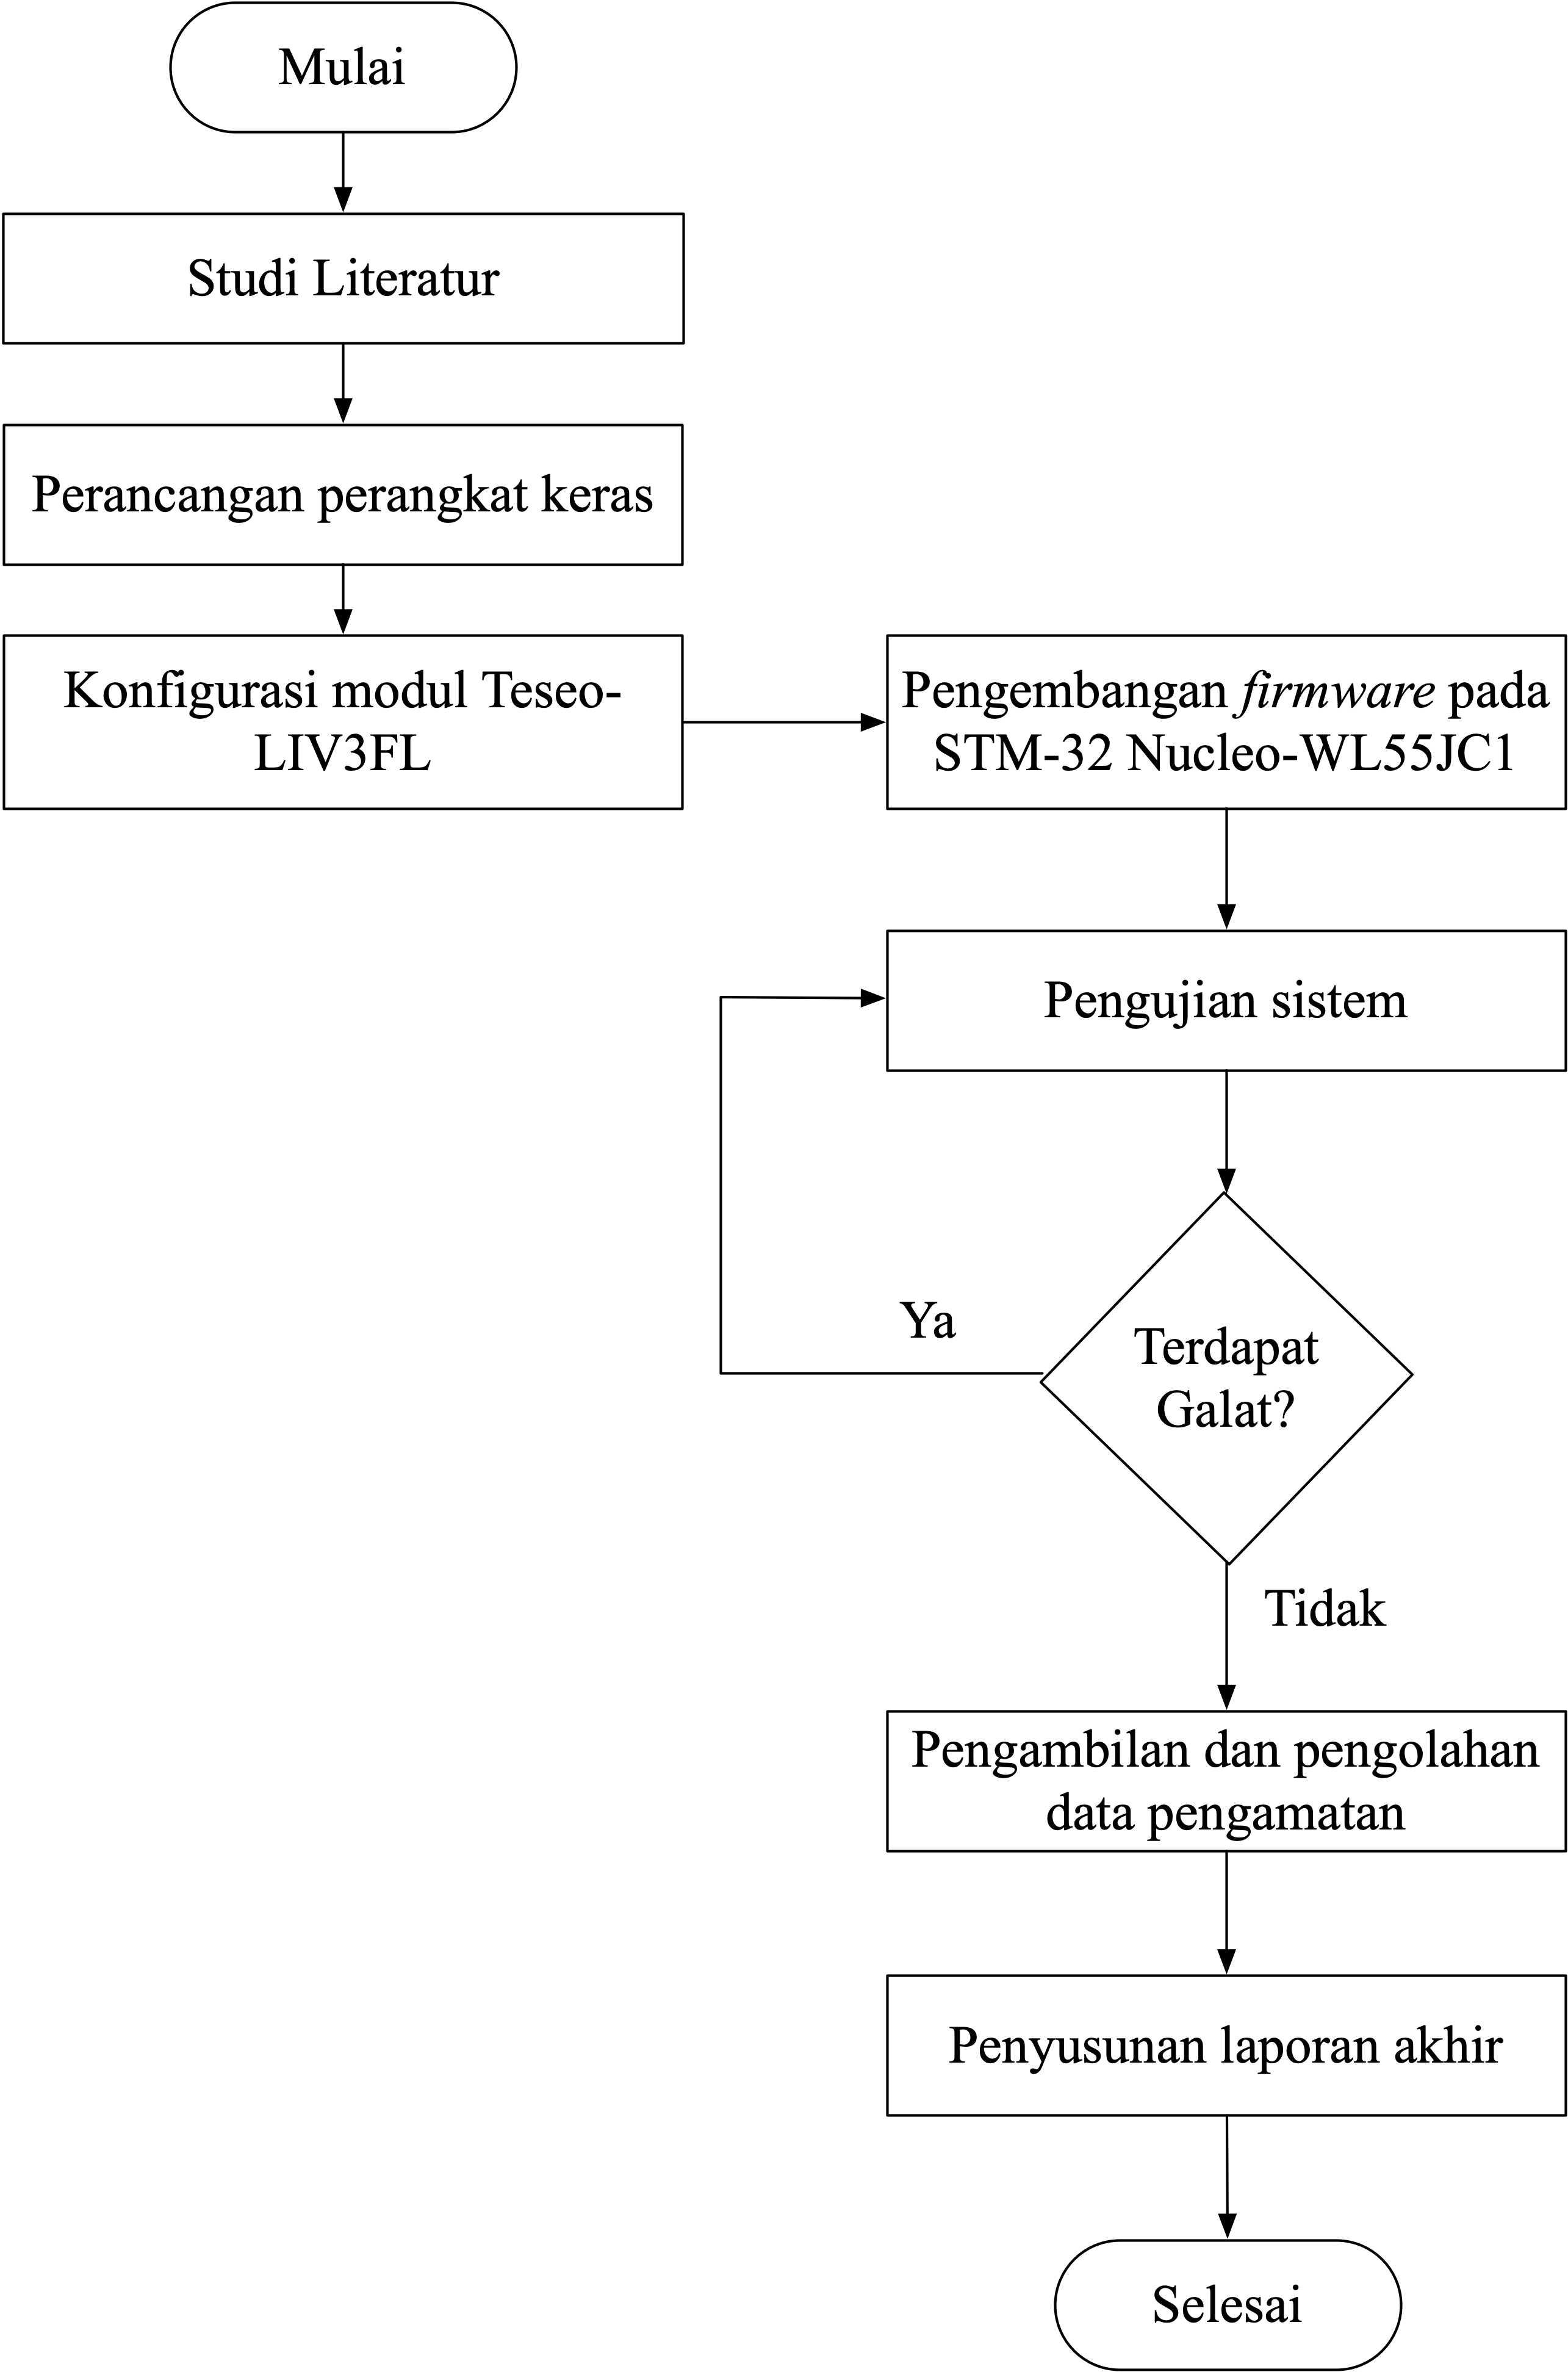
\includegraphics[width=10.5cm]{contents/chapter-3/diagram-alir-penelitian.png}
	\caption{Diagram Alir Penelitian}
	\label{Fig: diagram-alir-penelitian}
\end{figure}

\section{Studi Literatur}
Tahap studi literatur merupakan bagian penting dalam proses penelitian, karena melalui tahap ini penulis dapat memperoleh pemahaman yang lebih baik mengenai topik penelitian. Studi literatur dilakukan dengan mengumpulkan berbagai materi sebagai acuan dalam melakukan penelitian, seperti artikel dan jurnal ilmiah, laporan penelitian sebelumnya, situs \textit{web}, dan dokumentasi perangkat yang digunakan. Dalam tahapan ini, penulis juga berusaha memperoleh informasi terbaru dan relevan terhadap topik penelitian. Selain itu, tahap studi literatur juga dapat membantu penulis memperoleh keahlian yang diperlukan untuk melakukan penelitian, terutama dalam memahami dan menggunakan perangkat atau alat yang digunakan dalam penelitian. 

\begin{figure}[H]
	\centering
	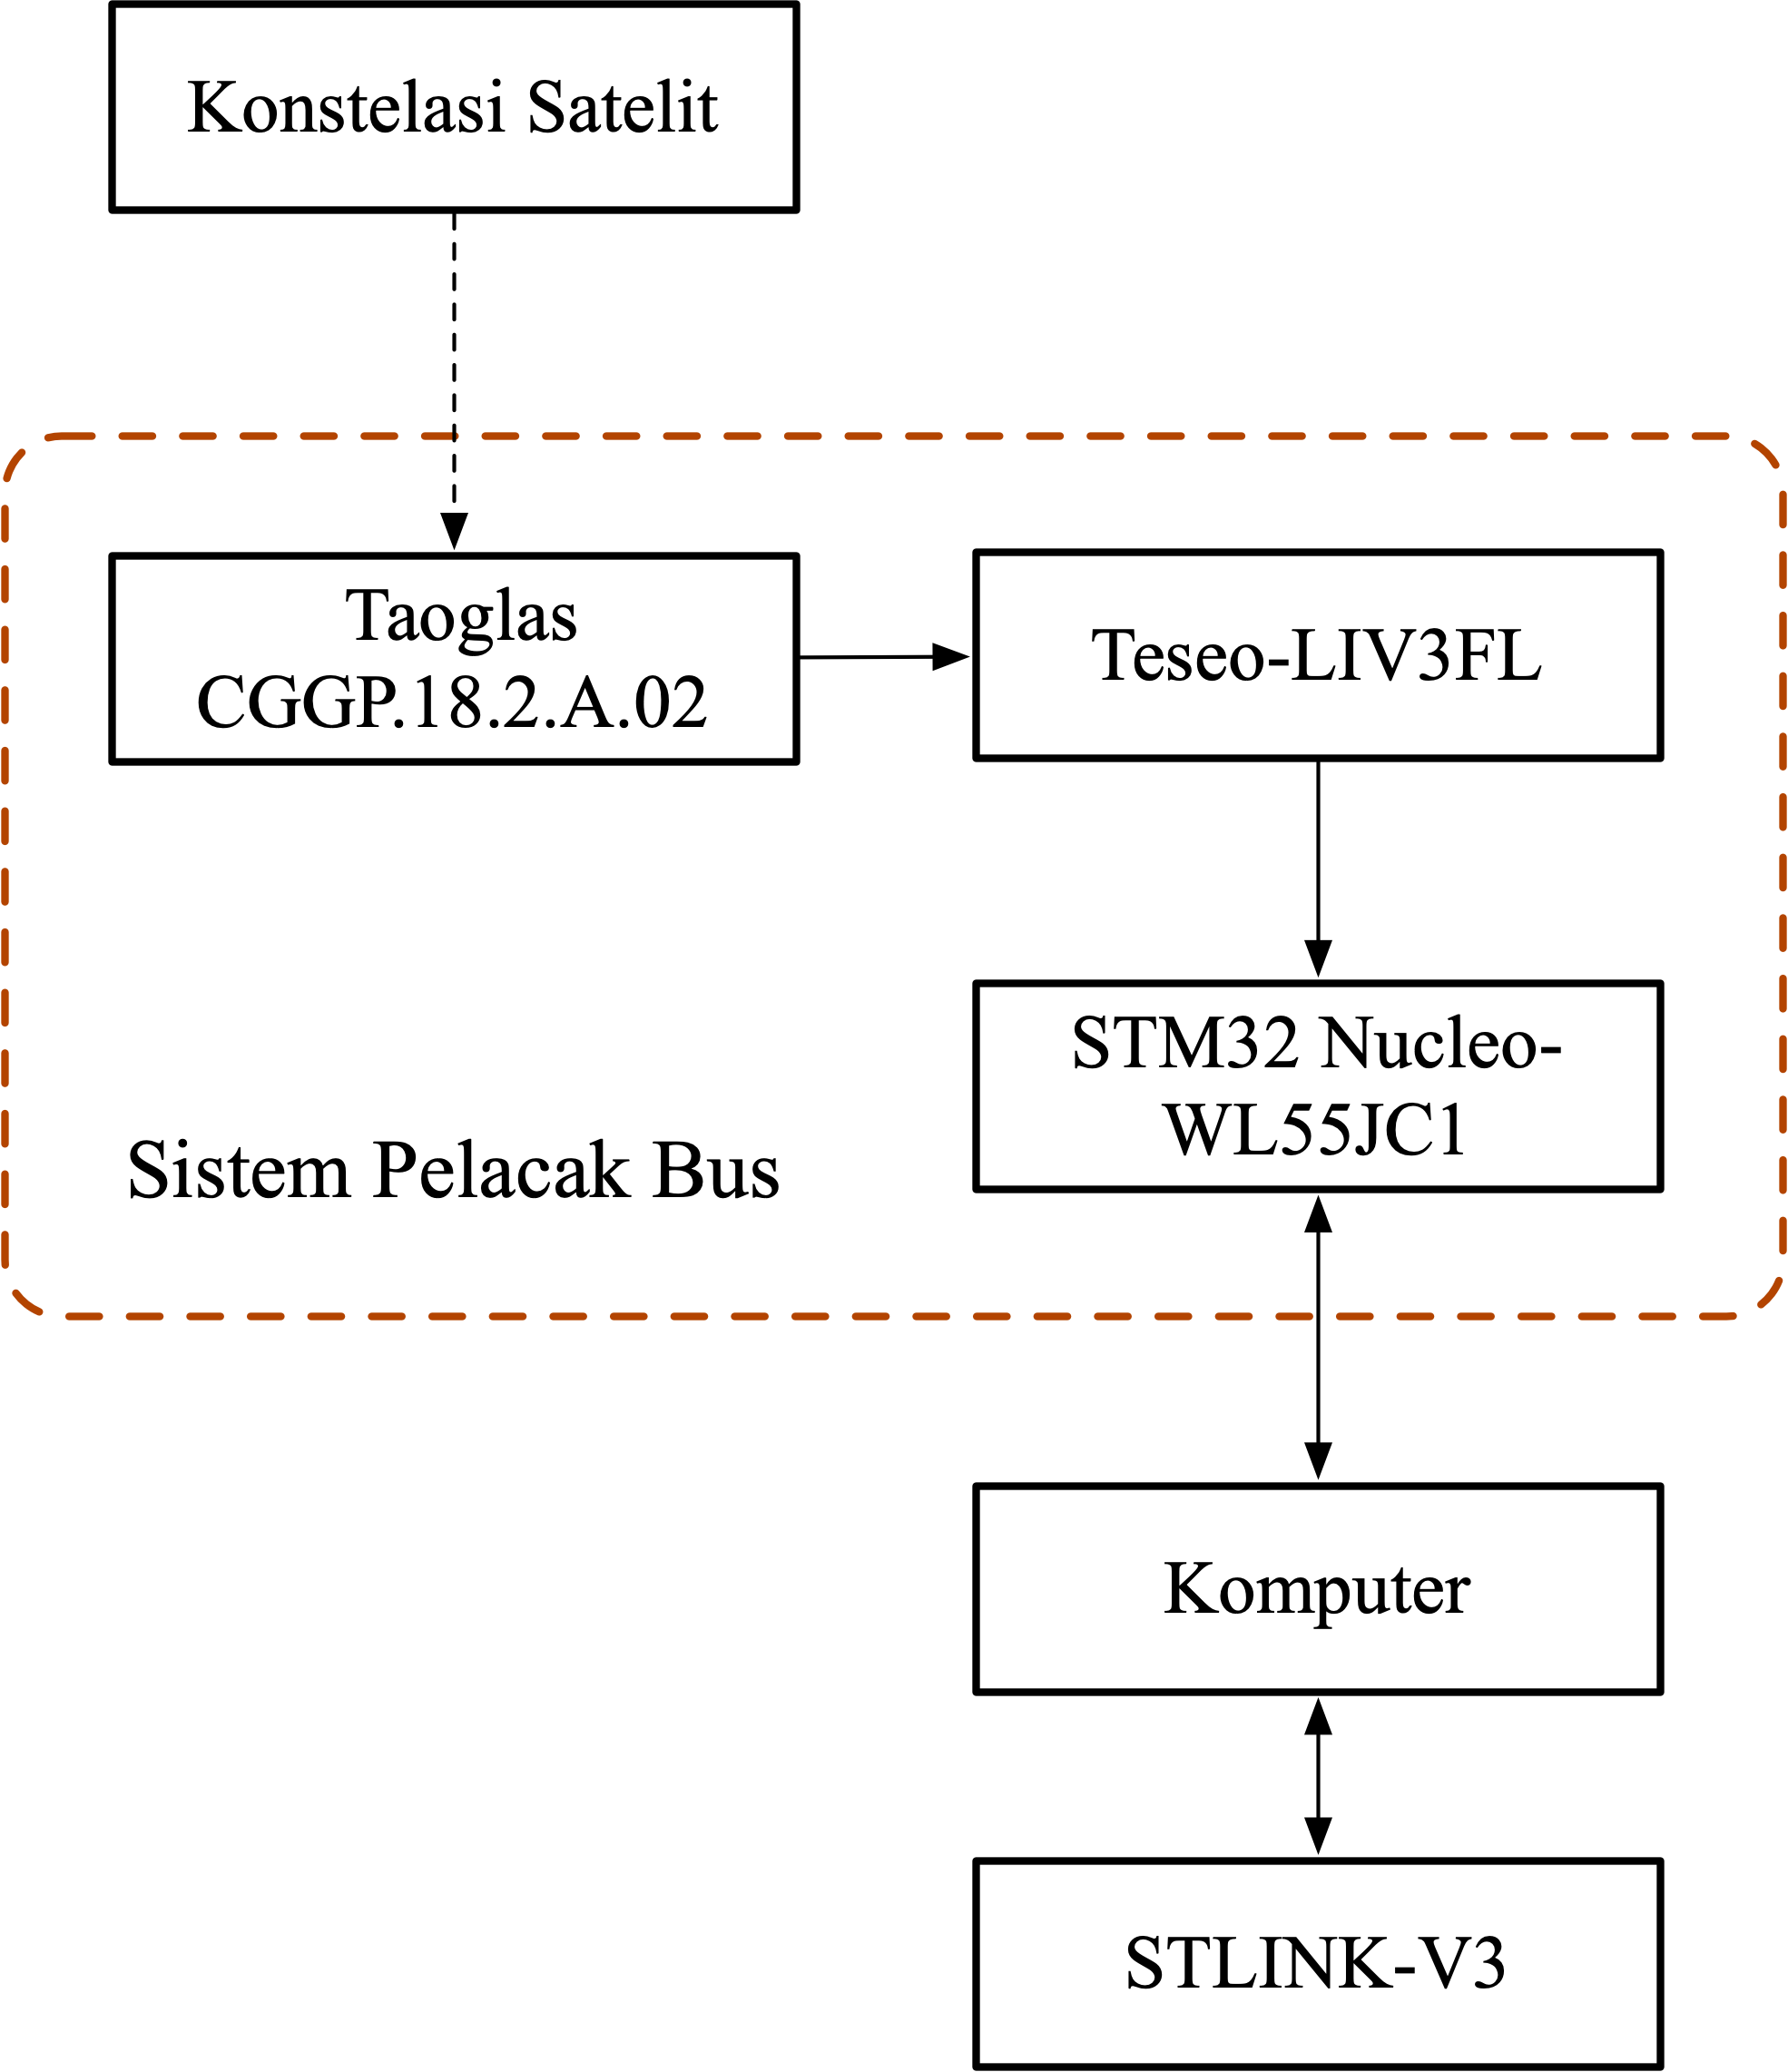
\includegraphics[width=11cm]{contents/chapter-3/system-overview.png}
	\caption{Ikhtisar Sistem}
	\label{Fig: system-overview}
\end{figure}

\section{Perancangan Perangkat Keras}
Rancangan purwarupa sistem digambarkan ditunjukan oleh ikhtisar sistem pada gambar Gambar  \ref{Fig: system-overview}. Fokus penelitian ini adalah pada perancangan firmware di STM32 saja.  Modul GNSS Teseo\hyp{}LIV3FL yang digunakan pada penelitian ini memiliki kemampuan yang sangat baik dalam menangkap isyarat satelit dan memproses informasi lokasi. Hal ini didukung oleh teknologi GNSS \textit{multi-constellation} yang diterapkan pada modul ini, yaitu GPS, GLONASS, Galileo, BeiDou, dan QZSS. Dengan teknologi ini, modul Teseo\hyp{}LIV3FL dapat menangkap isyarat satelit dari berbagai konstelasi dan meningkatkan akurasi posisi secara signifikan.

Komunikasi antara modul Teseo\hyp{}LIV3FL dan mikrokontroler dilakukan menggunakan protokol UART dengan \textit{baud rate} 9600 bps. Protokol UART dipilih karena implementasinya yang sederhana dan umum digunakan pada berbagai perangkat mikrokontroler. Selain itu, \textit{baud rate} yang dipilih juga disesuaikan dengan konfigurasi modul Teseo\hyp{}LIV3FL dalam mengirimkan data.

Untuk mempermudah pengembangan dan pengujian sistem, digunakan \textit{development board} STM32 Nucleo-WL55JC1 yang sudah terintegrasi dengan mikrokontroler STM32WL55. \textit{Development board} ini juga sudah dilengkapi dengan STLINK-V3 yang memungkinkan untuk mengunggah \textit{firmware} ke mikrokontroler dengan mudah melalui koneksi \textit{micro} USB pada \textit{board}. Hal ini mempermudah proses pengembangan dan pengujian sistem secara keseluruhan.

Agar modul Teseo\hyp{}LIV3FL dapat menentukan posisi dengan akurat, dibutuhkan informasi satelit yang cukup. Informasi ini diperoleh dari isyarat GNSS yang ditangkap oleh antena. Oleh karena itu, pada penelitian ini digunakan antena Abracon APARM1804-SG3.

\begin{figure}[H]
	\centering
	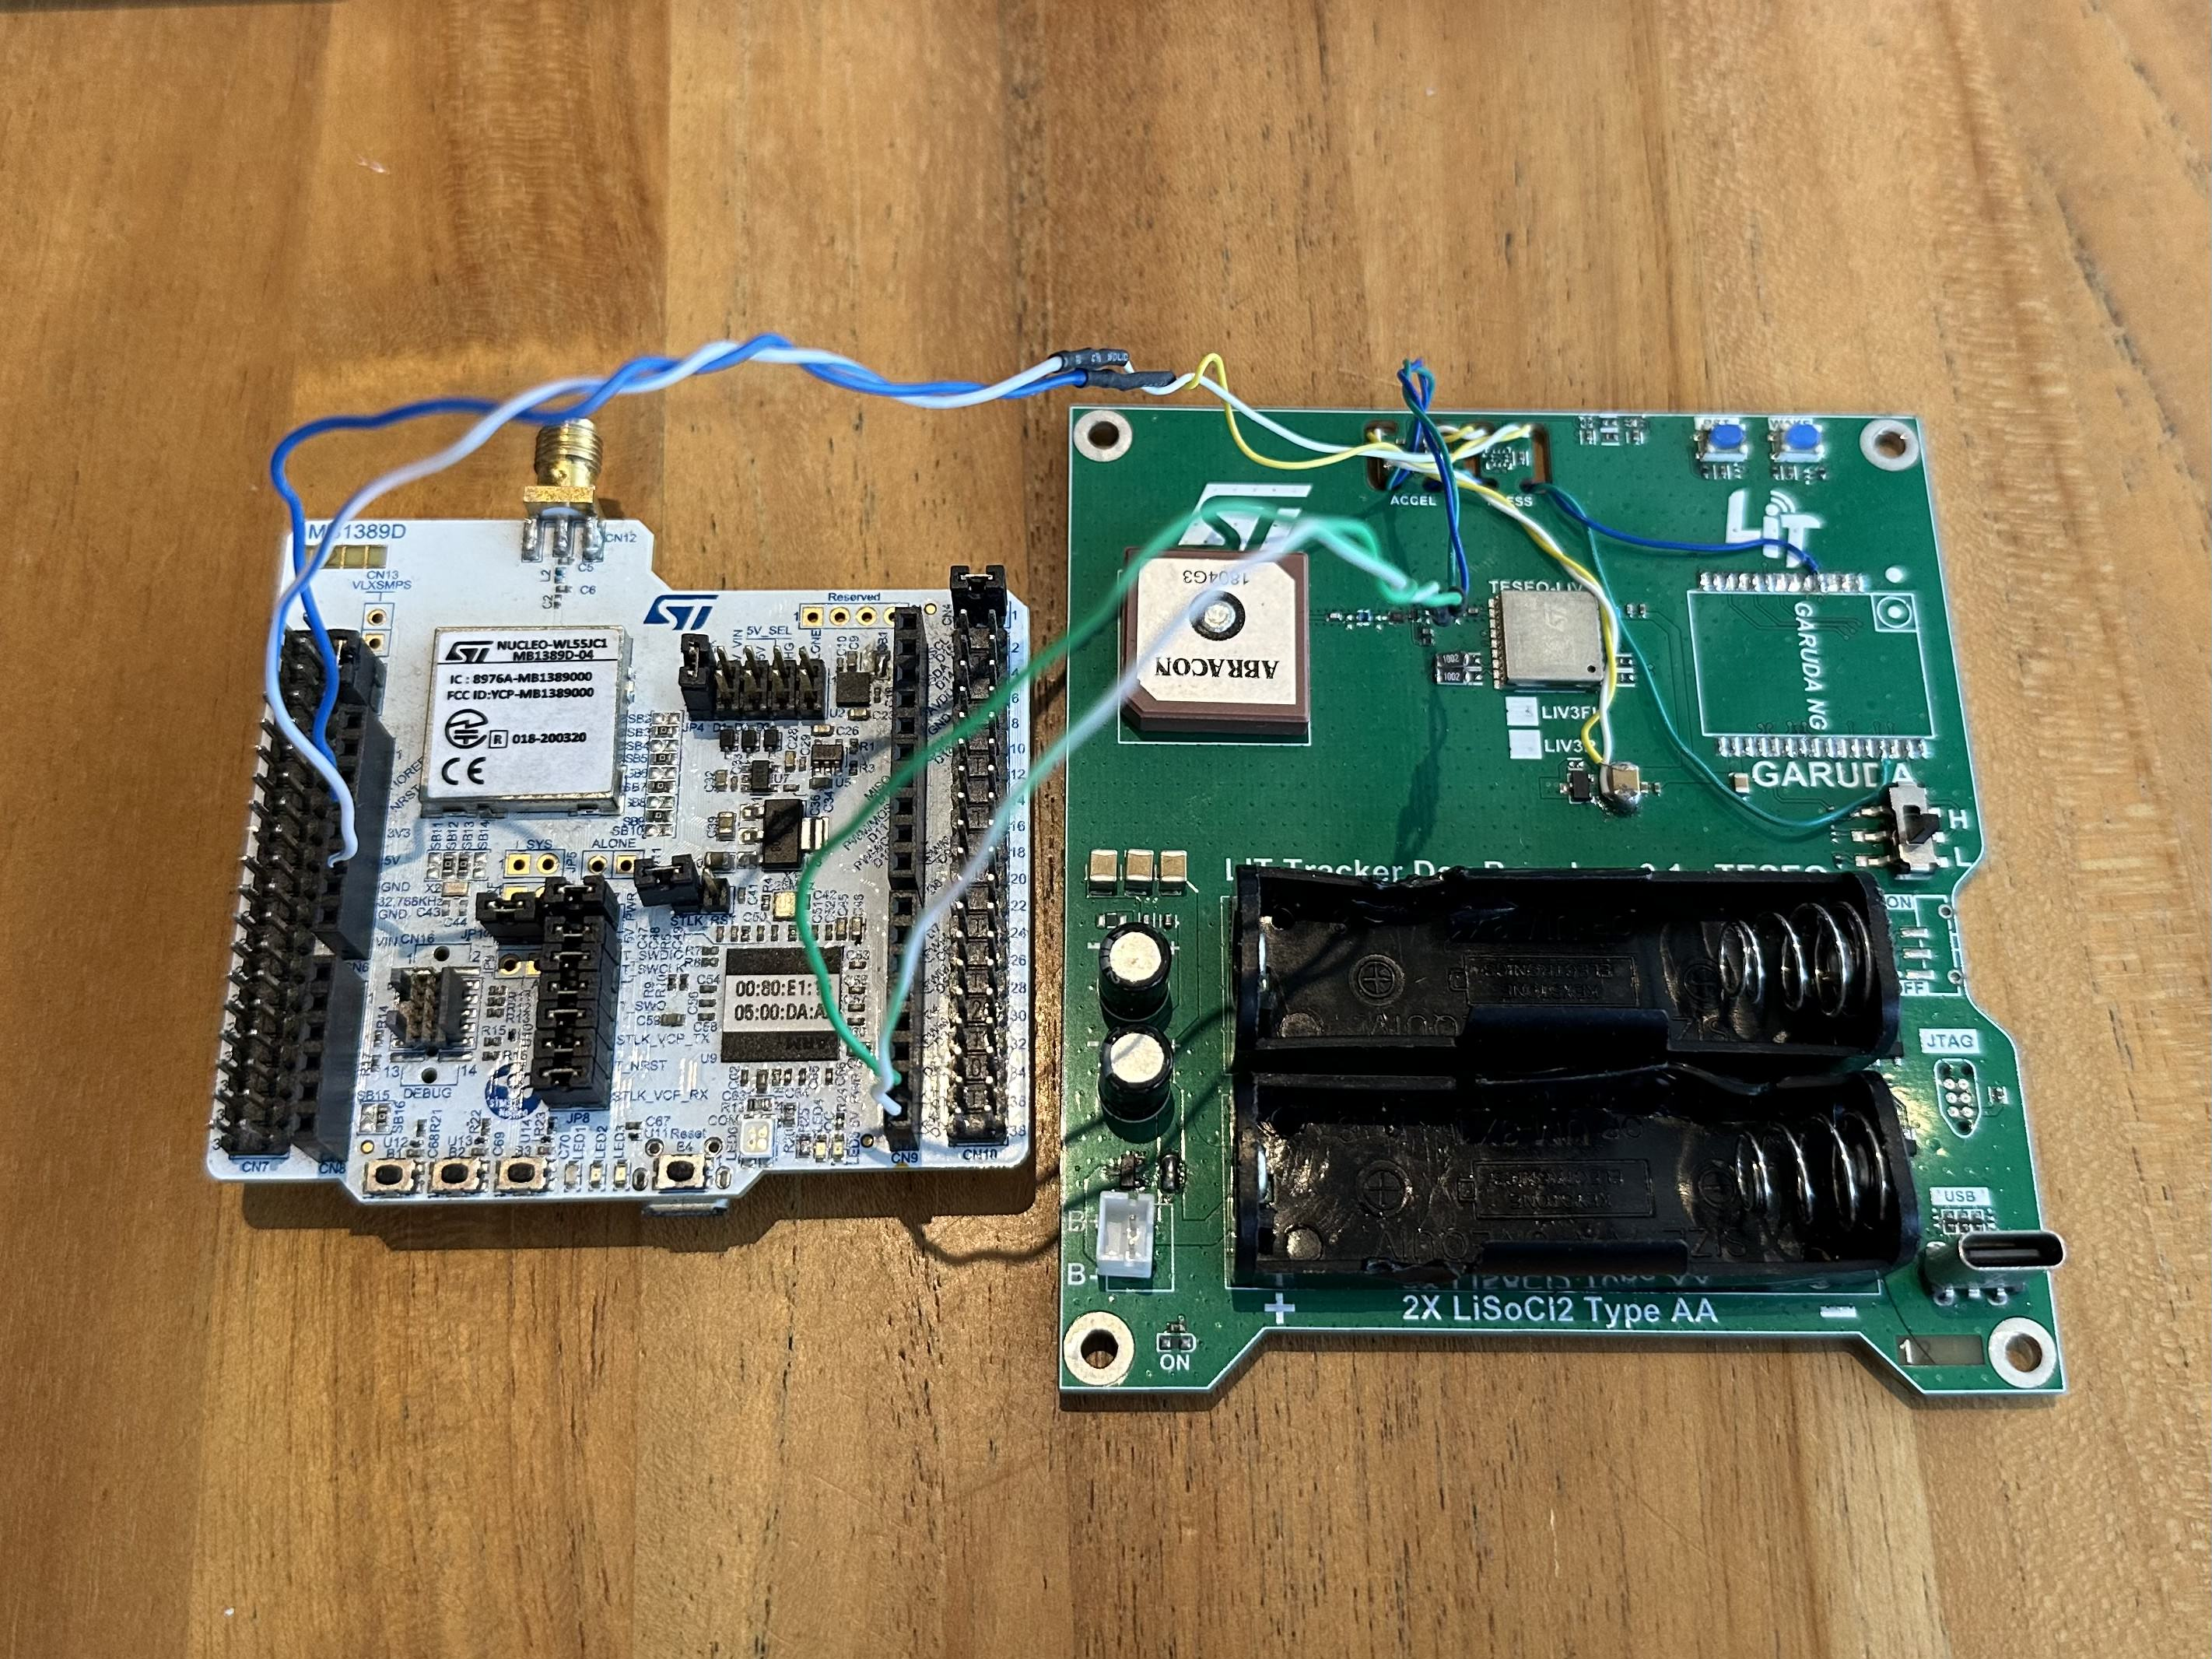
\includegraphics[width=9cm]{contents/chapter-3/purwarupa.jpg}
	\caption{Purwarupa Perangkat Keras}
	\label{Fig: purwarupa-alat}
\end{figure}

Untuk memudahkan integrasi antara modul Teseo\hyp{}LIV3FL dan antena Abracon APARM1804-SG3, keduanya sudah disolder pada satu papan yang disediakan oleh PT Lunar Inovasi Teknologi. Purwarupa dari perangkat keras ditunjukkan pada Gambar 3.3 yang menunjukkan desain dan komponen-komponen yang terpasang pada papan sirkuit tersebut.

\section{Konfigurasi pada Modul Teseo\hyp{}LIV3FL}
Dalam pengoperasian modul Teseo\hyp{}LIV3FL, konfigurasi merupakan salah satu elemen penting yang harus diperhatikan. Konfigurasi pada modul Teseo\hyp{}LIV3FL dikelompokan dalam bentuk blok data yang direpresentasikan dalam tiga digit ID. Digit pertama pada setiap ID merepresentasikan tipe parameter yang terdapat pada blok tersebut, sedangkan dua digit lainnya digunakan untuk membedakan parameter lainnya dalam tipe tersebut. Selama sistem berjalan, terdapat tiga blok konfigurasi yang mungkin dijalankan. Konfigurasi tersebut adalah:

\begin{enumerate}
	\item \textbf{Konfigurasi saat ini} berisi konfigurasi dari setiap blok saat ini disimpan pada RAM. Ketika modul diaktifkan ia akan memuat konfigurasi yang tersimpan pada \textit{non-volatile memory} (NVM) atau konfigurasi bawaan pabrik yang tertanam.
	\item \textbf{Konfigurasi bawaan} disimpan pada \textit{read only memory} (ROM). Konfigurasi ini akan dimuat ketika tidak ada konfigurasi valid pada NVM.
	\item \textbf{Konfigurasi NVM} berisi parameter yang telah dimodifikasi dan disimpan oleh pengguna.
\end{enumerate}

Selain CDB, pengguna juga dapat melakukan konfigurasi dengan menggunakan \textit{firmware configuration command}. Metode ini memungkinkan pengguna untuk mengatur berbagai CBD-ID dengan satu perintah saja. Sehingga, pengguna tidak perlu melakukan konfigurasi satu per satu pada setiap blok konfigurasi. \textit{Firmware configuration command} juga memungkinkan pengguna untuk melakukan pengaturan konfigurasi pada NVM secara langsung. Metode ini sangat berguna jika pengguna ingin mengatur konfigurasi dengan cepat.

\subsection{Konfigurasi \textit{Multi-constellation}}
Modul Teseo\hyp{}LIV3FL memiliki kemampuan untuk menerima isyarat dari lebih dari satu konstelasi GNSS atau biasa disebut sebagai \textit{multi-constellation}. Dalam kondisi bawaan, modul GNSS hanya menggunakan isyarat dari satu jenis konstelasi, seperti GPS. Namun, dengan kemampuan \textit{multi-constellation} pada modul Teseo\hyp{}LIV3FL, maka memungkinkan untuk menerima dan mengolah isyarat dari beberapa jenis konstelasi GNSS sekaligus, seperti GPS, GLONASS, Galileo, BeiDou, dan QZSS.
 
Keunggulan dari penggunaan \textit{multi-constellation} pada modul Teseo\hyp{}LIV3FL adalah dapat meningkatkan akurasi dari data posisi dan waktu yang dihasilkan oleh modul. Hal ini disebabkan karena dengan menerima isyarat dari beberapa konstelasi GNSS, maka modul dapat memperbaiki ketidakakuratan yang terjadi pada satu konstelasi dengan menggunakan informasi dari konstelasi lain \cite{An2020}.
 
\begin{figure}[H]
	\centering
	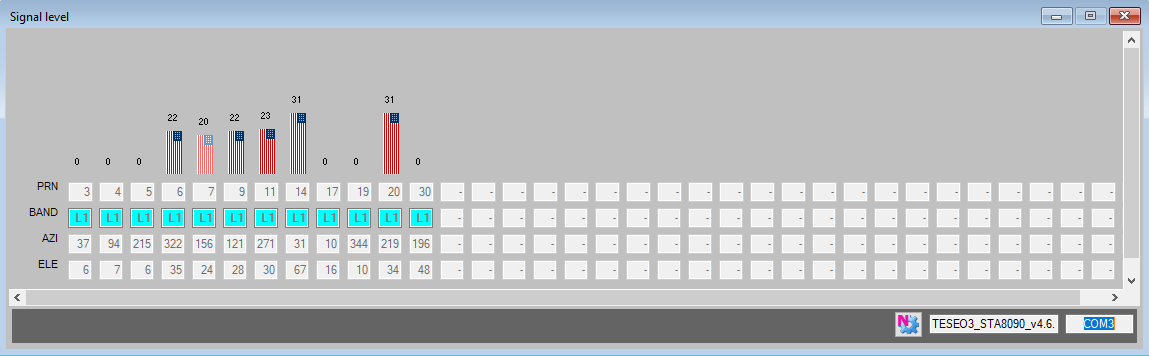
\includegraphics[width=14cm]{contents/chapter-3/setting-konstelasi/sebelum-konfigurasi.png}
	\caption{Isyarat yang Digunakan oleh Teseo\hyp{}LIV3FL Sebelum Dilakukan Konfigurasi}
	\label{Fig: sebelum-konfigurasi}
\end{figure}

 Untuk memudahkan proses konfigurasi konstelasi pada modul Teseo\hyp{}LIV3FL, pengguna dapat menggunakan aplikasi Teseo-Suite. Aplikasi ini memungkinkan pengguna untuk mengunggah konfigurasi ke \textit{non-volatile memory} pada modul Teseo\hyp{}LIV3FL. Selain itu, aplikasi Teseo-Suite juga dilengkapi dengan fitur untuk meninjau isyarat GNSS yang diterima dan digunakan oleh modul Teseo\hyp{}LIV3FL. Sebelum dilakukan konfigurasi, aplikasi Teseo-Suite dapat menunjukkan konstelasi mana saja yang digunakan oleh modul Teseo\hyp{}LIV3FL, seperti yang ditunjukkan pada Gambar \ref{Fig: sebelum-konfigurasi} terlihat bahwa hanya GPS yang digunakan sebelum dilakukan konfigurasi.
 
 \begin{figure}[H]
	\centering
	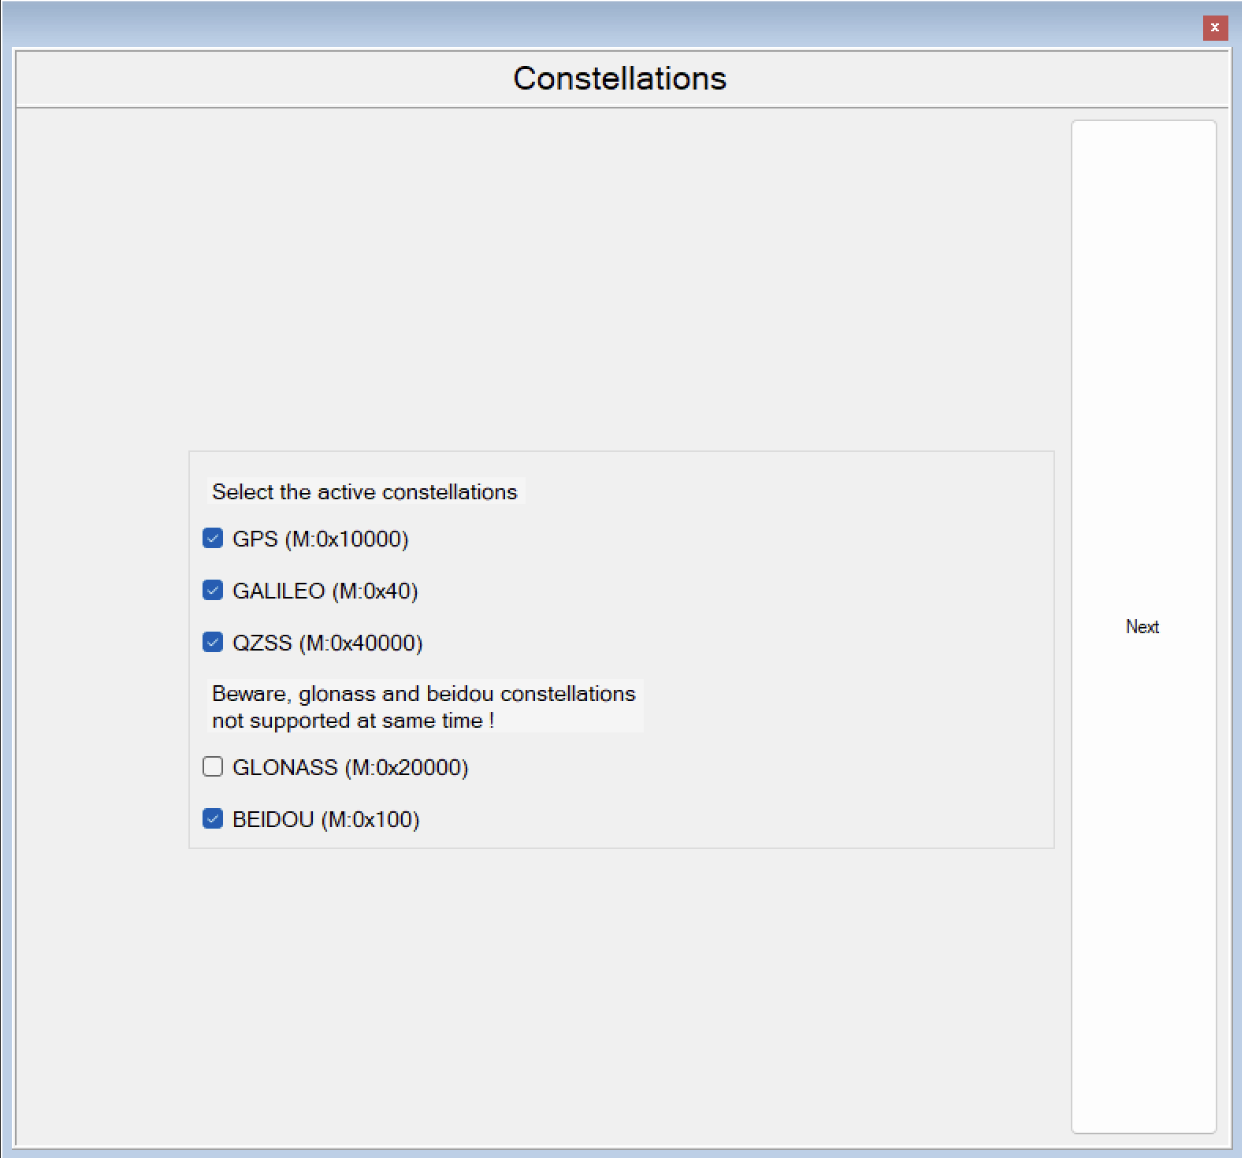
\includegraphics[width=10cm]{contents/chapter-3/setting-konstelasi/pilih-konfigurasi.png}
	\caption{Tampilan Teseo-Suite untuk Pemilihan Konstelasi}
	\label{Fig: pilih-konstelasi}
\end{figure}

Konfigurasi konstelasi yang akan digunakan dilakukan dengan membuka menu \textit{configuration wizards} dan memilih opsi \textit{constellation}. Akan terbuka jendela baru berisi \textit{constellation} seperti ditunjukan oleh Gambar \ref{Fig: pilih-konstelasi}. Pada penelitian ini akan digunakan empat konstelasi, yaitu GPS, BeiDou, QZSS, dan Galileo.

\begin{figure}[H]
	\centering
	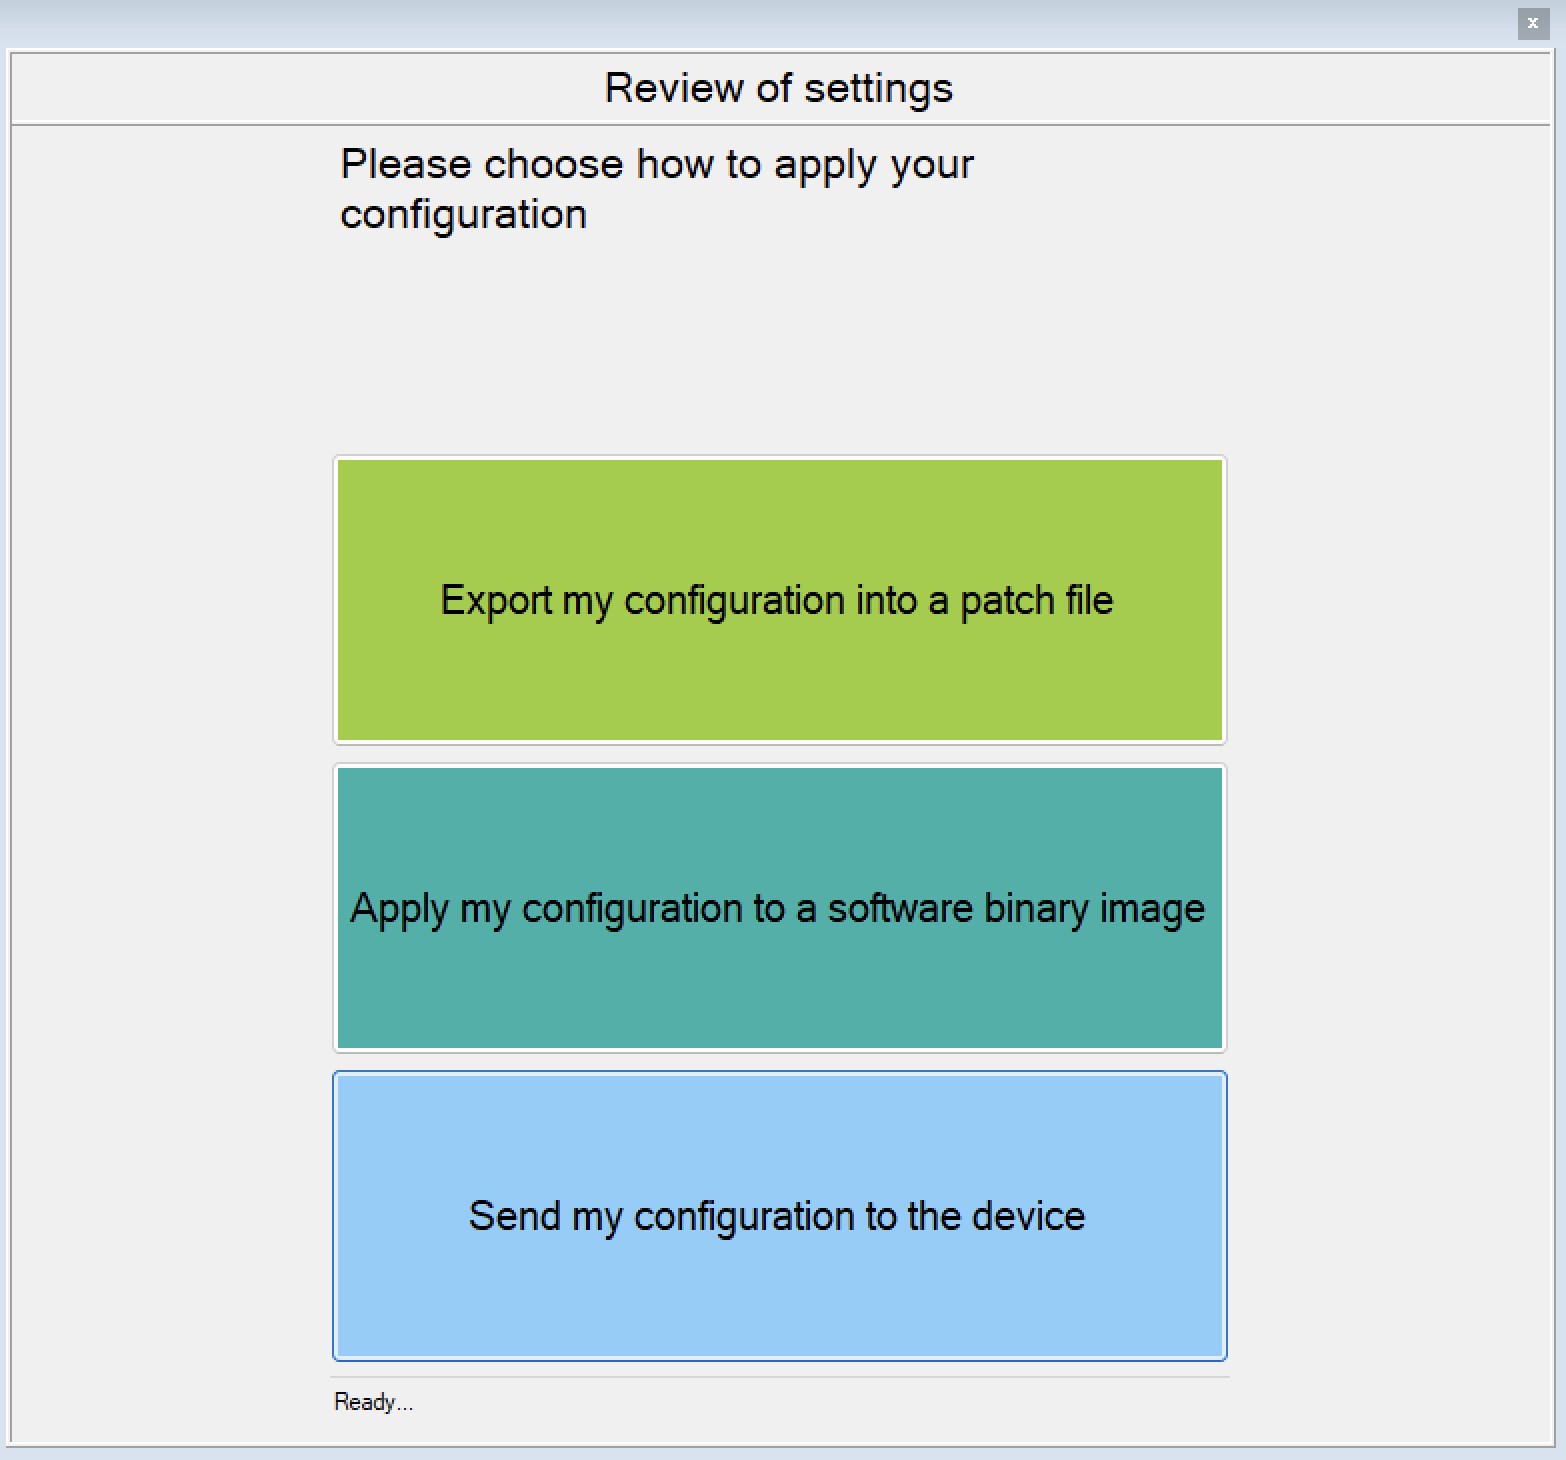
\includegraphics[width=10cm]{contents/chapter-3/setting-konstelasi/kirim-konfigurasi.png}
	\caption{Tampilan Teseo-Suite untuk Mengirimkan Konfigurasi}
	\label{Fig: kirim-konstelasi}
\end{figure}

Setelah konfigurasi yang dipilih pada aplikasi Teseo-Suite sudah benar, langkah selanjutnya yang harus dilakukan adalah mengeklik tombol \textit{send my configuration to the device}, seperti yang ditunjukkan pada Gambar \ref{Fig: kirim-konstelasi}. Aplikasi Teseo-Suite akan mengirimkan perintah berikut ke modul GNSS.

\begin{verbatim}
	$PSTMSETPAR,1200,E70000
	$PSTMSETPAR,1200,C50000
	$PSTMSETPAR,1227,3C0
	$PSTMSAVEPAR
\end{verbatim}

Terdapat dua CDB-ID yang akan dikonfigurasikan, yaitu CDB-ID 200 dan CDB-ID 227. CDB-ID 200 memiliki fungsi untuk mengatur konstelasi GPS dan QZSS, sementara CDB-ID 227 digunakan untuk mengatur konstelasi BeiDou dan Galileo. Dalam konteks ini, perintah yang dimaksud adalah \$PSTMSETPAR. Agar perubahan konfigurasi yang telah dilakukan dapat tersimpan dengan baik dan tidak hilang, maka diperlukan penggunaan perintah \$PSTMSAVEPAR. Perintah ini berfungsi untuk menyimpan konfigurasi yang telah diubah sebelumnya dan mengamankannya agar tidak terhapus saat pengaturan ulang sistem. 

\begin{figure}[H]
	\centering
	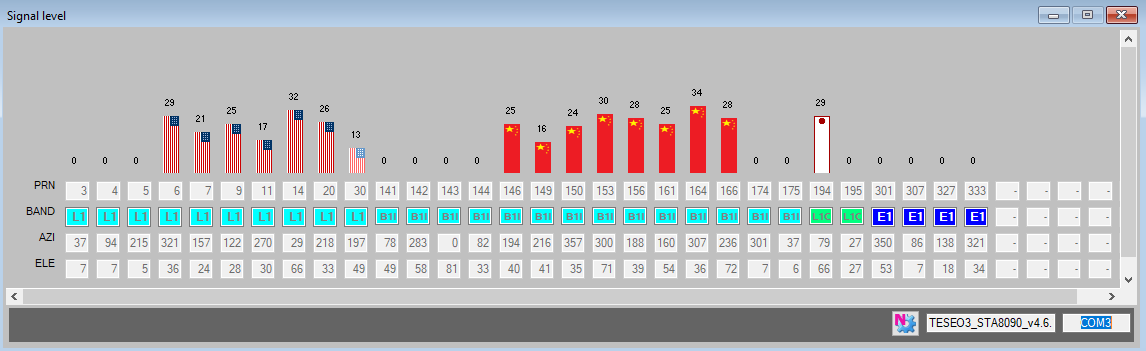
\includegraphics[width=14cm]{contents/chapter-3/setting-konstelasi/setelah-konfigurasi.png}
	\caption{Isyarat yang Digunakan oleh Teseo\hyp{}LIV3FL Setelah Dilakukan Konfigurasi}
	\label{Fig: setelah-konfigurasi}
\end{figure}

Setelah berhasil mengunggah konfigurasi yang telah dibuat sebelumnya, modul Teseo\hyp{}LIV3FL akan menggunakan tiga konstelasi tambahan yang telah diaktifkan. Konfigurasi yang telah diunggah akan memastikan bahwa modul GNSS menggunakan konstelasi yang diinginkan agar dapat memberikan data yang lebih akurat dan tepat waktu. Seperti yang ditunjukkan pada Gambar \ref{Fig: setelah-konfigurasi}, setelah konfigurasi berhasil diunggah, telihat bahwa modul Teseo\hyp{}LIV3FL akan menggunakan empat buah konstelasi, yaitu GPS, BeiDou, QZSS, dan Galileo. 

\begin{figure}[H]
	\centering
	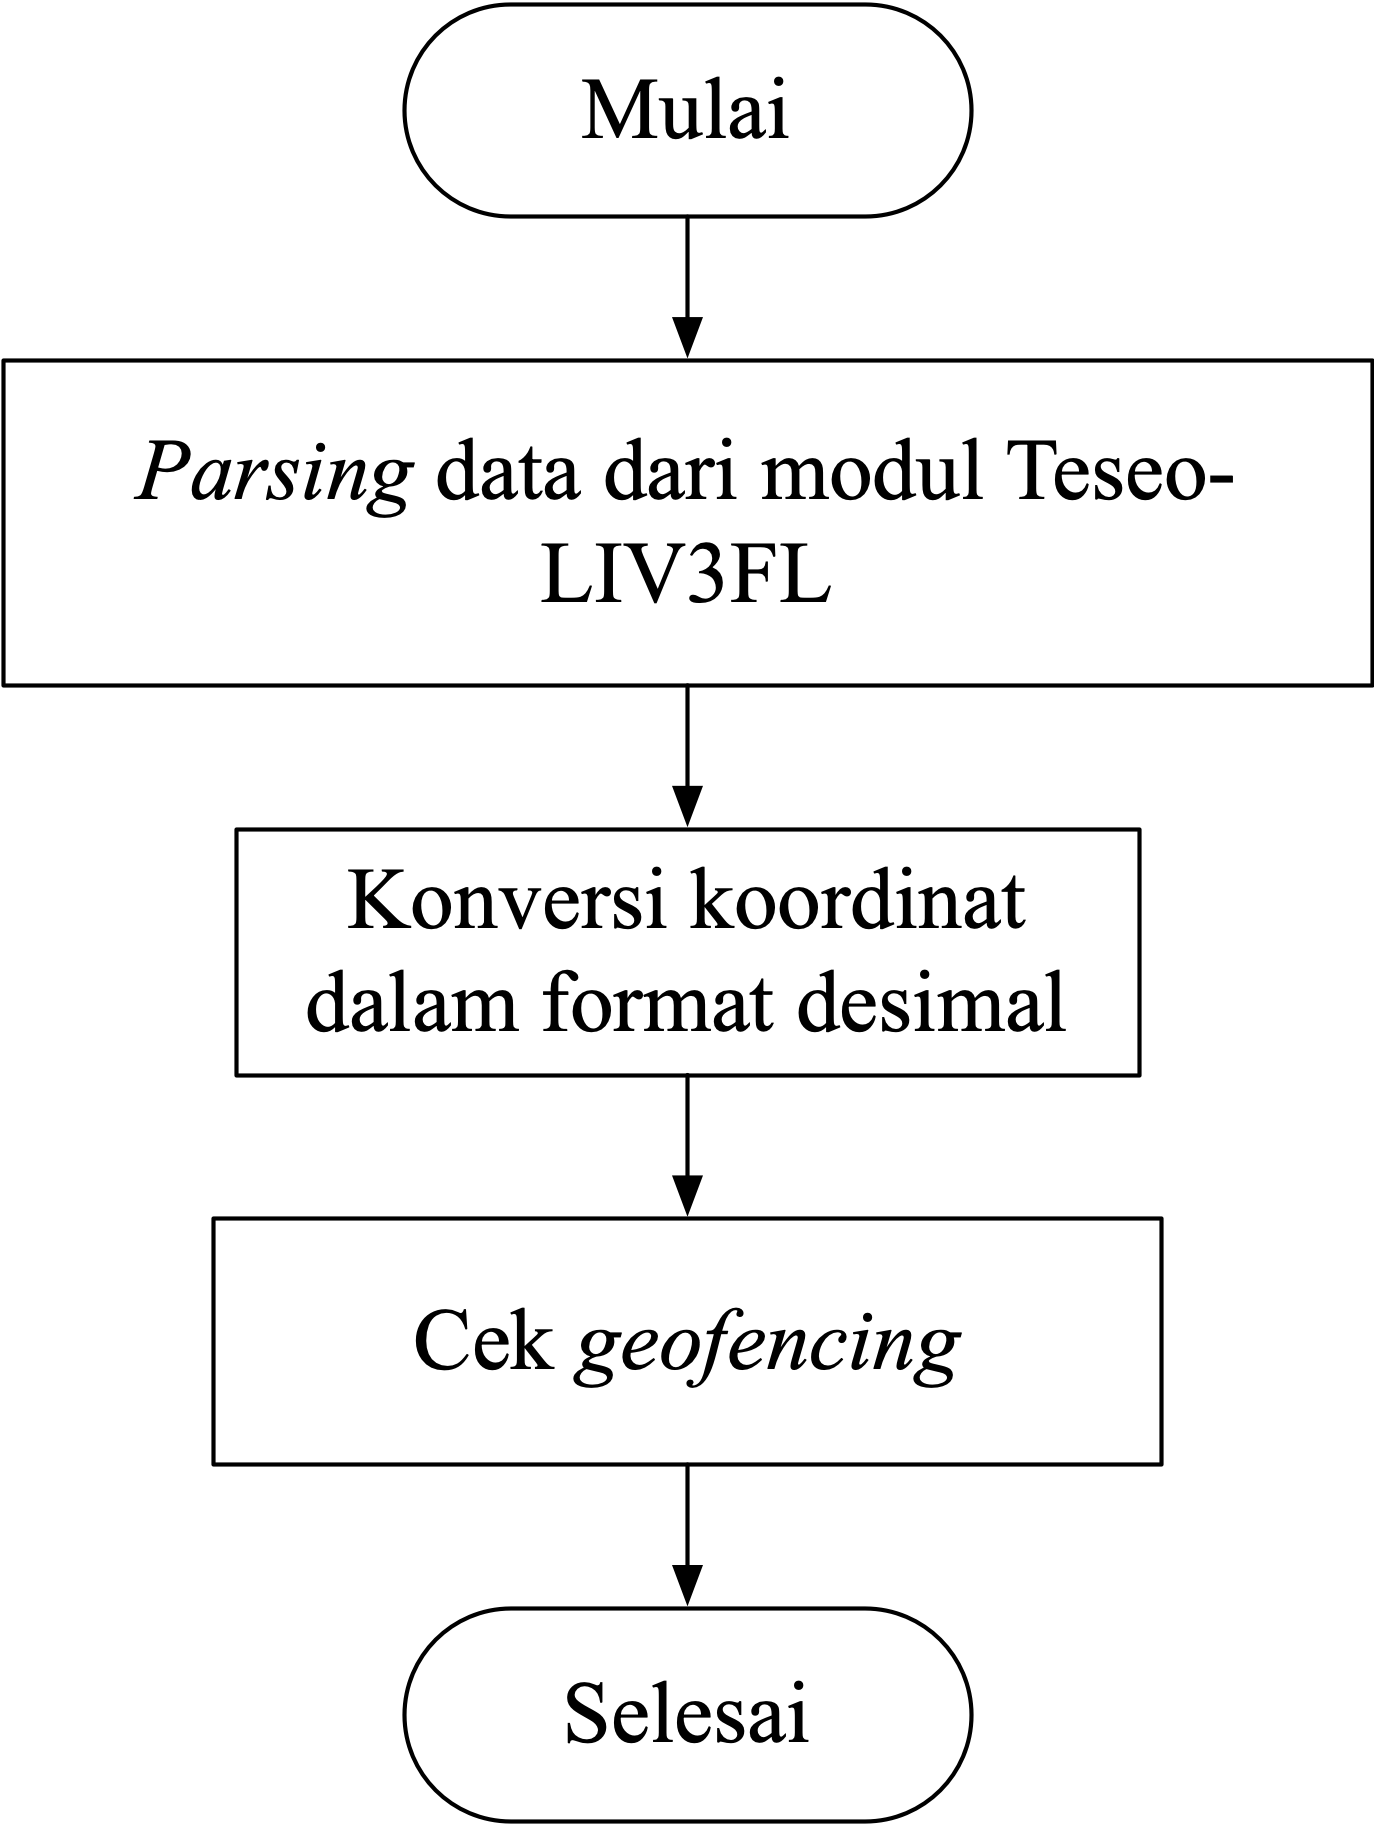
\includegraphics[width=6cm]{contents/chapter-3/firmware-diagram.png}
	\caption{Diagram Alir \textit{Firmware}}
	\label{Fig: flowchart-firmware}
\end{figure}

\section{Pengembangan \textit{Firmware} Mikrokontroler}
Pengembangan \textit{firmware} dilakukan dengan menggunakan STM32Cube IDE dan menggunakan bahasa pemrograman C. Untuk mempermudah pengembangan maka tahapan pengembangan dibagi menjadi tiga bagian kecil. Tiga bagian kecil tersebut tersebut adalah:
\begin{enumerate}
	\item Penguraian kalimat NMEA untuk ekstraksi data dari setiap kalimat NMEA yang digunakan. Tahap ini bertujuan untuk membaca dan memproses data GPS yang diterima dari satelit dan mengubahnya menjadi informasi yang bisa diproses oleh sistem.
	\item Konversi koordinat dari bentuk ddmm.mmm ke derajat desimal untuk mempermudah proses selanjutnya. Koordinat yang diterima dari satelit dalam format ddmm.mmm harus dikonversi menjadi format derajat desimal agar mudah diproses oleh sistem.
	\item Algoritma \textit{geofence} untuk menentukan apakah letak bus berada di dalam area kampus UGM atau tidak. Tahap ini bertujuan untuk menentukan apakah posisi bus saat ini berada di dalam area kampus UGM atau tidak, dengan membandingkan koordinat bus dengan koordinat area kampus yang telah ditentukan sebelumnya.
\end{enumerate}
diagram alir \textit{firmware} secara garis besar ditunjukan oleh Gambar \ref{Fig: flowchart-firmware}.

Sebelum melakukan pengembangan lebih lanjut, ada beberapa langkah yang perlu dilakukan untuk mempersiapkan \textit{development board} STM32. Salah satu langkah yang penting adalah melakukan konfigurasi pin pada \textit{board} tersebut. Untuk melakukan konfigurasi ini, dapat dilakukan dengan menyunting berkas .ioc yang berbasis STM32Cube MX. Dalam proses konfigurasi ini, perlu diaktifkan USART1 agar STM32 dapat berkomunikasi dengan modul Teseo\hyp{}LIV3FL dengan \textit{baud rate} 9600 Bps. Selain itu, USART2 juga perlu diaktifkan agar \textit{development board} dapat berkomunikasi dengan komputer dengan \textit{baud rate} 115200 Bps.

\begin{longtblr}[caption = {Struktur Pesan \$GNGSA}]{
	width = \linewidth,
	colspec = {Q[125]Q[817]},
	row{1} = {c},
	cell{2}{1} = {c},
	cell{3}{1} = {c},
	cell{4}{1} = {c},
	cell{5}{1} = {c},
	cell{6}{1} = {c},
	cell{7}{1} = {c},
	cell{8}{1} = {c},
	cell{9}{1} = {c},
	hline{1-2,10} = {-}{},
}
\textbf{Struktur} & \textbf{Deskripsi}                                                             \\
header            & \textit{Header} pesan \\
mode M/A          & A jika otomatis dan M jika dipaksa untuk peroperasi pada mode 2D atau 3D       \\
mode 123          & 1 jika tidak ada fiksasi, 2 untuk mode 2D, dan 3 untuk mode 3D        \\
prn               & ID satelit yang digunakan (kosong jika dalam mode \textit{multi-constellation} \\
pdop              & Nilai PDOP                                                                     \\
hdop              & Nilai HDOP                                                                     \\
vdop              & Nilai VDOP                                                                     \\
chksum            & \textit{Checksum}dalam bentuk heksadesimal
\end{longtblr}

\begin{longtblr}[caption = {Struktur Pesan \$GPGGA}]{
width = \linewidth,
colspec = {Q[98]Q[717]},
row{1} = {c},
cell{2}{1} = {c},
cell{2}{3} = {c},
cell{3}{1} = {c},
cell{3}{3} = {c},
cell{4}{1} = {c},
cell{4}{3} = {c},
cell{5}{1} = {c},
cell{5}{3} = {c},
cell{6}{1} = {c},
cell{6}{3} = {c},
cell{7}{1} = {c},
cell{7}{3} = {c},
cell{8}{1} = {c},
cell{8}{3} = {c},
cell{9}{1} = {c},
cell{9}{3} = {c},
cell{10}{1} = {c},
cell{10}{3} = {c},
cell{11}{1} = {c},
cell{11}{3} = {c},
cell{12}{1} = {c},
cell{12}{3} = {c},
cell{13}{1} = {c},
cell{13}{3} = {c},
cell{14}{1} = {c},
cell{14}{3} = {c},
cell{15}{1} = {c},
cell{15}{3} = {c},
cell{16}{1} = {c},
cell{16}{3} = {c},
cell{17}{1} = {c},
cell{17}{3} = {c},
hline{1-2, 18} = {-}{},
}
\textbf{Struktur}   & \textbf{Deskripsi} \\
\texttt{header}     & \textit{Header} pesan\\
\texttt{utc}        & Waktu UTC dalam format hhmmss.ss \\
\texttt{lat}        & Garis lintang\\
\texttt{lat\_dir}   & Arah garis lintang\\
\texttt{lon}        & Garis bujur \\
\texttt{lon\_dir}   & Arah garis bujur \\
\texttt{quality}    & Kualitas fiksasi. Jika bernilai nol maka tidak \textit{valid}\\
\texttt{satelit}    & Jumlah satelit yang digunakan\\
\texttt{hdop}       & Nilai HDOP \\
\texttt{alt}        & Ketinggian antena dari permukaan laut\\
\texttt{a-units}    & Satuan dari ketinggian antena\\
\texttt{und} & Perbedaan ketinggian antara Geoid dengan elipsoid \\
\texttt{u-units}    & Satuan dari perbedaan ketinggian\\
\texttt{age}        & Umur dari koreksi data dalam sekon (kosong jika tidak ada data diferensial) \\
\texttt{stn-ID}     & Nomor pengidentifikasi stasiun referensi diferensial (kosong jika tidak ada data diferensial)\\
\texttt{chksum}     & \textit{Checksum} dalam bentuk heksadesimal   
\end{longtblr}

\subsection{Penguraian Kalimat NMEA}
Modul Teseo\hyp{}LIV3FL merupakan sebuah perangkat yang digunakan untuk mengirimkan data dalam format standar NMEA-0813 yang dimiliki oleh \textit{National Marine Electronics Association}. Standar NMEA-0813 sendiri memiliki beberapa format data yang dapat digunakan, namun pada penelitian ini hanya akan digunakan dua jenis kalimat NMEA, yaitu GPGGA yang berisi data tetap GNSS dan GNGSA yang berisi nilai DOP dari pembacaan. Dalam kalimat NMEA, setiap informasi dipisahkan oleh tanda koma dan asteris untuk memisahkan dengan \textit{checksum}. Struktur lebih detail mengenai kalimat GNGSA dan GPGGA dapat dilihat pada Tabel 3.1 dan Tabel 3.2, yang menunjukkan rincian dari setiap informasi dalam dua jenis kalimat tersebut.

\begin{figure}[H]
	\centering
	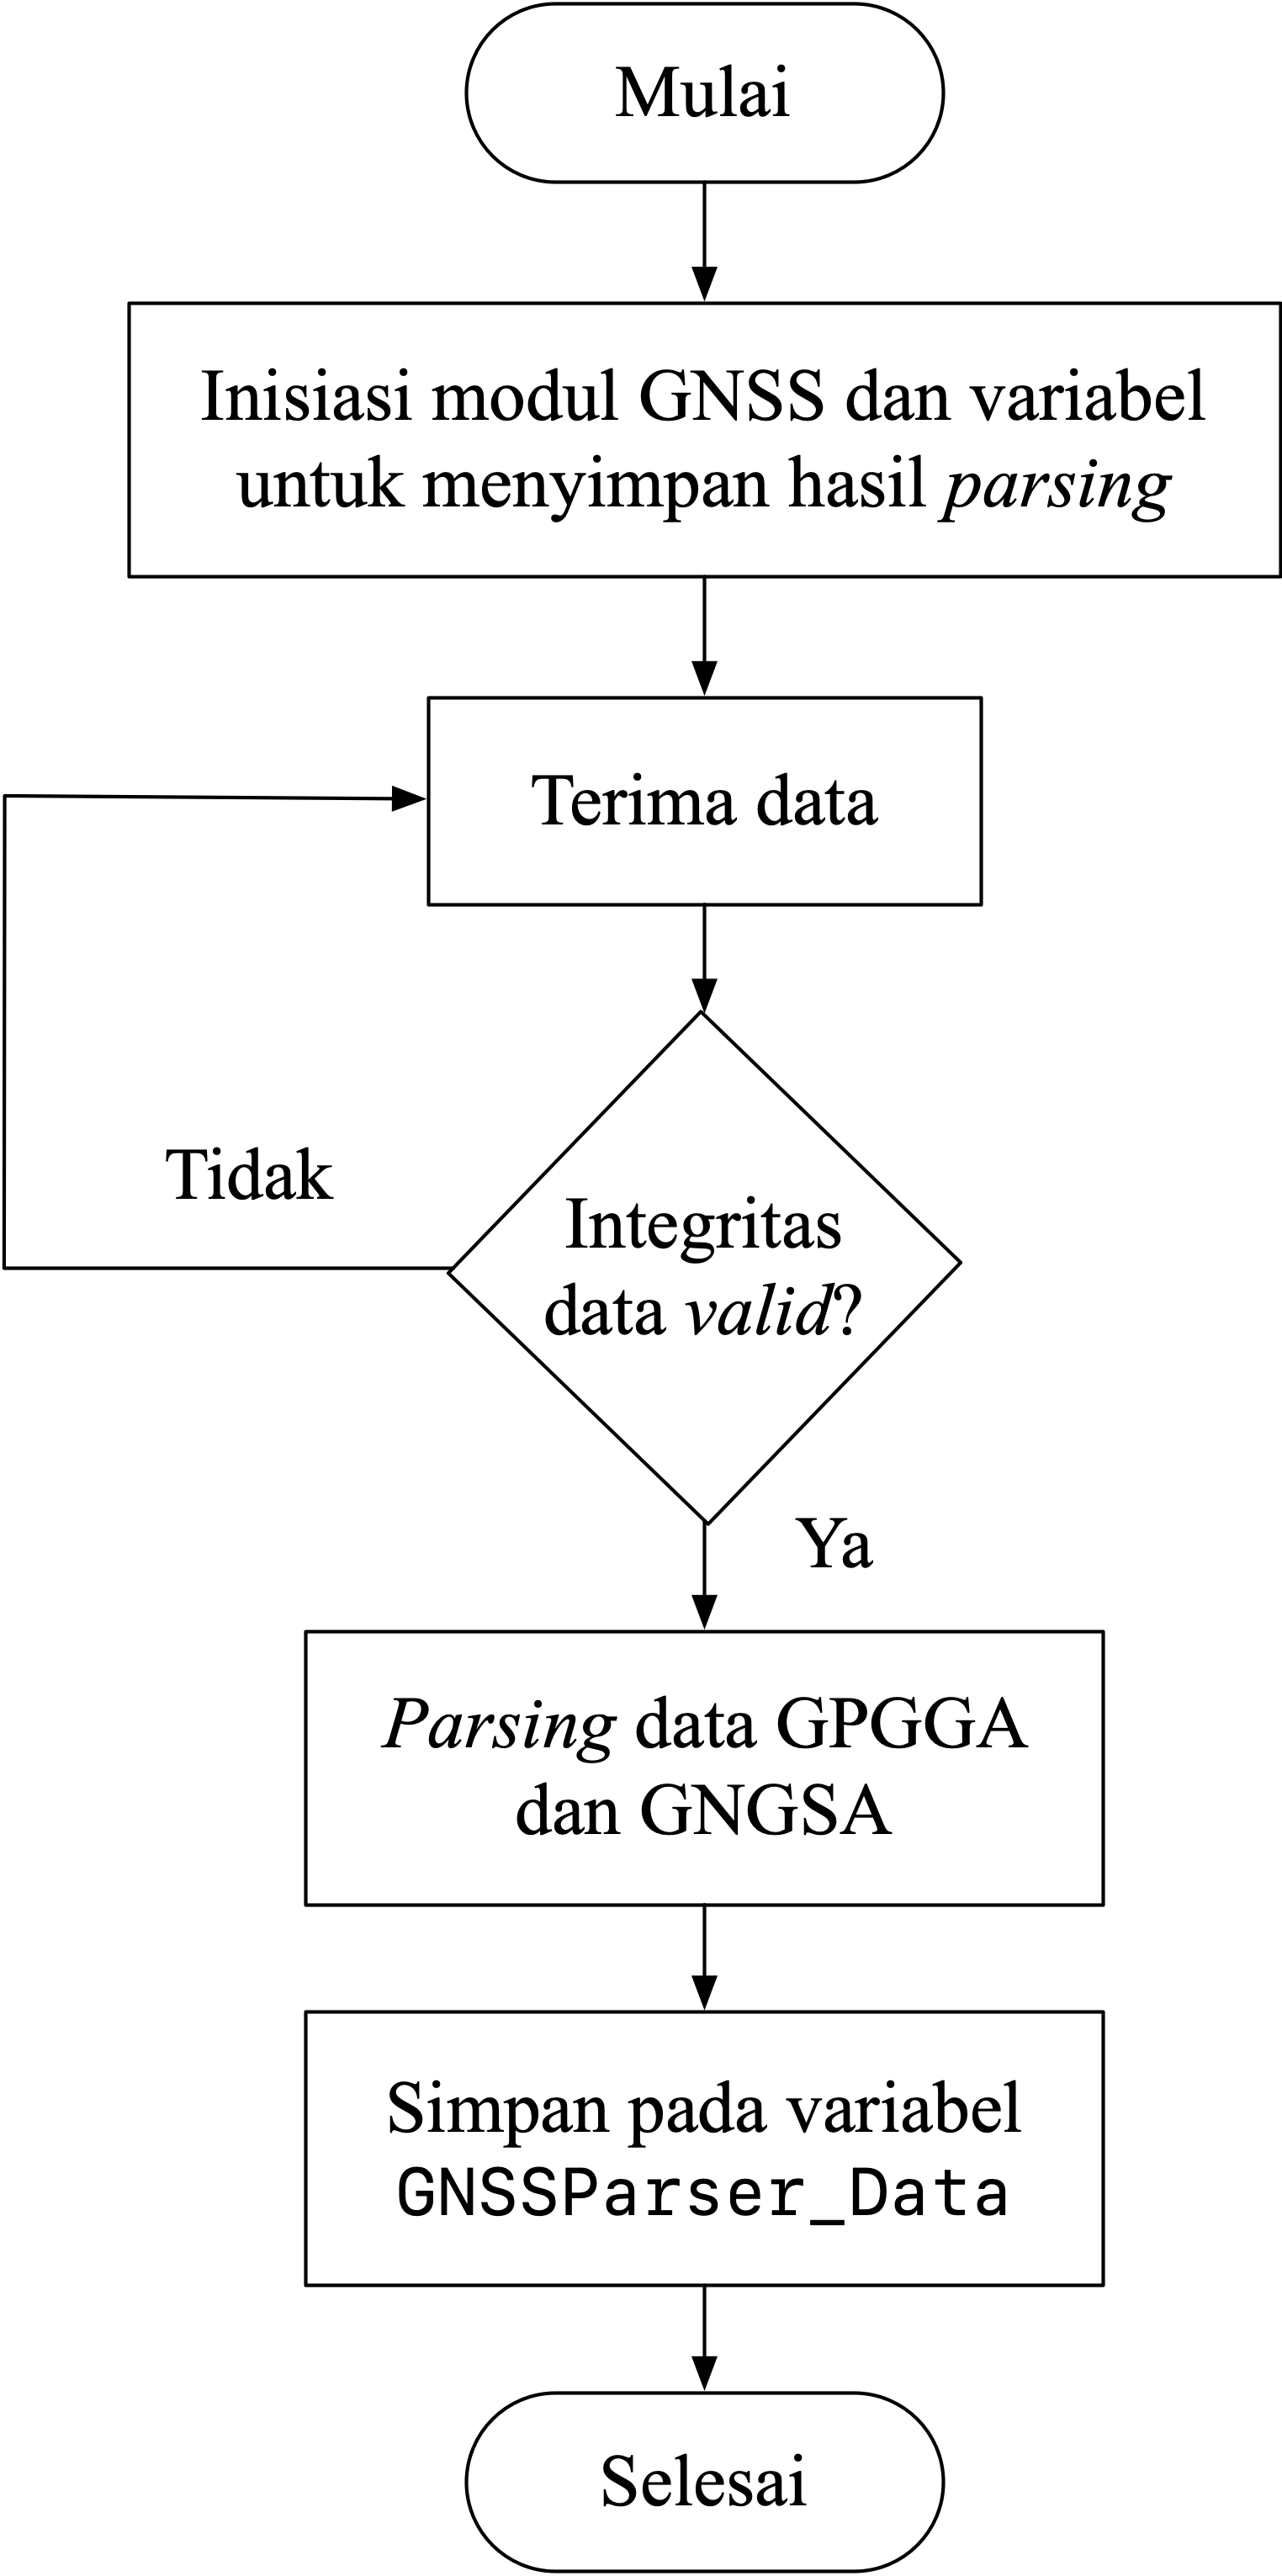
\includegraphics[width=6.5cm]{contents/chapter-3/diagram-parser.png}
	\caption{Diagram Alir Proses Penguraian Kalimat NMEA}
	\label{Fig: flowchart-parsing}
\end{figure}

Proses penguraian pada penelitian ini terdiri dari beberapa tahapan. Tahapan pertama adalah inisiasi perangkat GNSS dan variabel penyimpanan hasil penguraian. Selanjutnya, dilakukan akuisisi data dari modul Teseo\hyp{}LIV3FL yang mengirimkan data dalam format standar NMEA-0813. Tahapan selanjutnya adalah melakukan pengecekan \textit{sanity} untuk memeriksa integritas data yang diterima sebelum melakukan proses penguraian utama. Proses penguraian utama akan dilakukan pada data tersebut valid menurut hasil pengecekan \textit{sanity}. Terakhir, proses penguraian akan diakhiri dengan \textit{release} \textit{buffer} kalimat NMEA. Diagram alir proses penguraian dapat dilihat pada Gambar \ref{Fig: flowchart-parsing}, yang memperlihatkan tahapan-tahapan tersebut dalam bentuk diagram alir.

\subsubsection{Inisiasi}
Proses penguraian diawali dengan memuat pustaka-pustaka yang akan digunakan dalam pengembangan \textit{firmware}. Pustaka \texttt{<stdio.h>} menyediakan fungsi-fungsi untuk IO standar pada bahasa C, seperti \texttt{printf()} dan \texttt{scanf()}. Pustaka \texttt{<stdlib.h>} menyediakan fungsi-fungsi umum pada bahasa C, seperti alokasi memori, konversi tipe data, dan lain-lain. Pustaka \texttt{<string.h>} menyediakan fungsi-fungsi yang berkaitan dengan pengolahan \textit{string}, seperti \texttt{strcpy()} dan \texttt{strlen()}. Pustaka \texttt{<stdint.h>} menyediakan tipe data integer dengan ukuran yang terdefinisi secara pasti, seperti \texttt{uint8\_t} dan \texttt{int32\_t}. Pustaka \texttt{"teseo\_liv3f\_conf.h"} berisi konfigurasi khusus untuk modul Teseo\hyp{}LIV3FL. Pustaka \texttt{"custom\_gnss.h"} berisi definisi fungsi-fungsi khusus yang digunakan dalam pengolahan data GNSS, sementara \texttt{"stm32wlxx\_nucleo.h"} berisi definisi fungsi-fungsi yang digunakan untuk mengakses perangkat keras pada \textit{board} \texttt{STM32WLxx Nucleo}.

Jika seluruh pustaka yang dibutuhkan telah berhasil dimuat, fungsi \texttt{CUSTOM\_GNSS\_Init} akan dijalankan. Fungsi \texttt{CUSTOM\_GNSS\_Init} akan mengembalikan nilai dari variabel \texttt{ret} seperti ditunjukan oleh Algoritma \ref{alg: 3-custom_init}. Setelah itu, fungsi ini akan memanggil \texttt{TESEO\_LIV3F\_Probe()} untuk memeriksa apakah modul Teseo\hyp{}LIV3FL sudah terhubung dengan baik atau tidak. Jika modul GNSS sudah terhubung dengan baik maka fungsi akan mengembalikan nilai \texttt{BSP\_ERROR\_NONE}, sedangkan jika terdapat galat pada modul maka fungsi akan mengembalikan nilai \texttt{BSP\_ERROR\_NO\_INIT}.

\begin{algorithm}
	\caption{Fungsi \texttt{CUSTOM\_GNSS\_Init} pada \textit{Firmware}}
	\label{alg: 3-custom_init}
	\begin{algorithmic}[1]
	\Function{CUSTOM\_GNSS\_Init}{}
		\State \textbf{Declare} ret as int32\_t
		\State ret $\gets$ BSP\_ERROR\_NONE
		\\
		\If{\Call{TESEO\_LIV3F\_Probe}{} $\neq$ BSP\_ERROR\_NONE}
			\State ret $\gets$ BSP\_ERROR\_NO\_INIT
		\EndIf
		\\
		\State \textbf{return} ret
	\EndFunction
	\end{algorithmic}
\end{algorithm}

Setelah itu, fungsi \texttt{GNSS\_Parser\_Init} digunakan untuk inisiasi struktur \texttt{GNSSParser\_Data\_t} seperti ditunjukan oleh Algoritma \ref{alg: 3-main-func2}. Pada fungsi ini, struktur \texttt{gpgga\_data} dan \texttt{gsa\_data} diatur menjadi nol untuk menghindari galat atau hal tidak terduga lainnya. Struktur \texttt{gpgga\_data} berisi informasi mengenai waktu dalam bentuk UTC, koordinat di bidang datar, ketinggian, nilai HDOP, dan jumlah satelit yang digunakan. Di sisi lain, struktur \texttt{gsa\_data} berisi nilai akurasi GNSS yang lebih detail, yaitu HDOP, PDOP, dan VDOP. Jika proses inisiasi struktur berjalan dengan lancar, maka fungsi akan mengembalikan nilai \texttt{GNSS\_PARSER\_OK}. Namun, jika terdapat galat, maka fungsi akan mengembalikan nilai \texttt{GNSS\_PARSER\_ERROR}.

\begin{algorithm}
	\caption{Inisiasi Struktur \texttt{GNSSParser\_Data\_t} pada \textit{Firmware}}\label{alg: 3-main-func2}
	\begin{algorithmic}[1]
		\State GNSSParser\_Status\_t status, check;
		\State CUSTOM\_GNSS\_Msg\_t *gnssMsg;
		\\
		\State CUSTOM\_GNSS\_Init();
		\\
		\State GNSS\_PARSER\_Init(\&GNSSParser\_Data);
	\end{algorithmic}
\end{algorithm}

Apabila fungsi \texttt{CUSTOM\_GNSS\_Init} berhasil mengembalikan nilai \texttt{GNSS\_PARSER\_OK}, maka langkah selanjutnya adalah menerima data yang dikirimkan oleh modul Teseo\hyp{}LIV3FL. Hal ini dapat dilakukan dengan memanggil fungsi \texttt{CUSTOM\_GNSS\_GetMessage} seperti ditunjukan pada Algoritma \ref{alg: 3-main-func}. Data yang diterima kemudian disimpan pada variabel \texttt{gnssMsg}, yang berisi nilai dari \textit{buffer} serta panjangnya. Variabel \texttt{gnssMsg} ini akan berisi data yang akan diolah pada tahap selanjutnya.

\begin{algorithm}
	\caption{Memuat Pustaka pada \textit{Firmware}}
	\label{alg: 3-main-func}
	\begin{algorithmic}[1]
	\While{true}
		\State gnssMsg $\gets$ \Call{CUSTOM\_GNSS\_GetMessage}{}
		\\
		\If{gnssMsg = NULL}
			\State \textbf{continue}
		\EndIf
	\EndWhile	
	\end{algorithmic}
\end{algorithm}

\subsubsection{Cek Integritas Data}
Dalam pengiriman pesan, pesan yang diterima tidak selalu dalam keadaan sempurna. Terkadang sebagian karakter pada pesan hilang atau tercampur dengan karakter lainnya. Oleh karena itu, untuk memastikan bahwa pesan yang didapat adalah benar dan dapat diproses dengan baik, digunakan fungsi \texttt{GNSS\_PARSER\_CheckSanity} untuk memeriksa integritas data yang diterima. Sebelum melakukan proses pengecekan, nilai \textit{checksum} dari kalimat NMEA masih dalam bentuk heksadesimal sehingga perlu dilakukan konversi ke bentuk integer terlebih dahulu.

Setelah menerima pesan, proses pengecekan dilakukan dengan membandingkan nilai \textit{checksum} data yang diterima dengan nilai \textit{checksum} yang tertera pada kalimat NMEA. Penghitungan nilai \textit{checksum} dilakukan dengan mengenakan operasi XOR pada setiap \textit{bytes} yang berada di antara simbol "\$" dan "*". Jika hasil perhitungan \textit{checksum} pada kalimat NMEA sama dengan hasil perhitungan pada data yang diterima, maka fungsi akan mengembalikan nilai \texttt{GNSS\_PARSER\_OK} yang menandakan bahwa data telah lulus pengecekan integritas. Sebaliknya, jika terdapat perbedaan antara nilai \textit{checksum} pada kalimat NMEA dan data yang diterima, maka fungsi akan mengembalikan nilai \texttt{GNSS\_PARSER\_ERROR} yang menandakan adanya kesalahan atau ketidaksesuaian pada data yang diterima.

Implementasi fungsi \texttt{GNSS\_PARSER\_CheckSanity} untuk melakukan proses pengecekan integritas data dari kalimat NMEA ditunjukan oleh Algoritma \ref{alg: 3-nmea-checksum}.

\begin{algorithm}
	\caption{\textit{Checksum} Kalimat NMEA}
	\label{alg: 3-nmea-checksum}
	\begin{algorithmic}[1]
	\State checksum $\gets$ (char2int(pSentence[len-4U]) $<<$ 4) $|$ char2int(pSentence[len-3U])
	\State check $\gets$ 0
	\\
	\For{c $\gets$ 1U to (len-5U)}
		\State check $\gets$ (check XOR pSentence[c])
	\EndFor
	\\
	\If{check = checksum}
		\State ret $\gets$ GNSS\_PARSER\_OK
	\Else
		\State ret $\gets$ GNSS\_PARSER\_ERROR
	\EndIf
	\\
	\State \textbf{return} ret			
	\end{algorithmic}
\end{algorithm}

\subsubsection{Proses Penguraian Utama}
Modul GNSS Teseo\hyp{}LIV3FL mengirimkan tiga belas kalimat NMEA standar dan empat kalimat NMEA milik STMicroelectronics yang diawali oleh \$PSTM. Karena pada penelitian hanya digunakan kalimat \$GPGGA dan GNGSA maka diperlukan suatu mekanisme untuk memeriksa apakah kalimat yang diterima termasuk di antara salah satu yang digunakan. Proses penguraian kalimat \$GPGGA dan \$GNGSA dibuat dalam dua fungsi yang berbeda untuk mempermudah pengembangan. 

Fungsi \texttt{NMEA\_ParseGPGGA} digunakan untuk menguraikan kalimat \$GPGGA. Variabel \texttt{app} diinisiasikan sebagai larik yang berisi \textit{string}. Bagian perulangan dilakukan hingga \textit{line break} atau karakter \texttt{\textbackslash n}. Setelah perulangan selesai, variabel \texttt{app} akan berisi seluruh bagian yang terdapat pada kalimat NMEA. Variabel \texttt{i} digunakan sebagai indeks dari perulangan, sedangkan \texttt{j} dan \texttt{k} sebagai indeks dari variabel \texttt{app}. Nilai \texttt{valid\_msg} akan bernilai benar jika kalimat NMEA yang diterima diawali dengan \$GPGGA. Sebaliknya, perulangan akan dihentikan jika pesan NMEA yang diterima tidak diawali dengan \$GPGGA.

Jika karakter pada iterasi saat ini adalah asteris atau tanda koma maka karakter terakhir akan diatur sebagai \textit{null terminator}. Selain itu, variabel \texttt{k} akan diatur kembali menjadi nol dan \texttt{j} ditambahkan satu. Sebaliknya, jika karakter pada iterasi saat ini bukan asteris atau tanda koma maka karakter tersebut akan disimpan dalam variabel \texttt{app} dengan indeks \texttt{j} dan \texttt{k}. Bagian perulangan \textit{parsing} kalimat \$GPGGA ditunjukan oleh Algoritma \ref{alg: 3-parse-gpgga}.

\begin{algorithm}[H]
	\caption{\textit{Parsing} Kalimat \$GPGGA pada \textit{Firmware}}
	\label{alg: 3-parse-gpgga}
	\begin{algorithmic}[1]
	\State \textbf{Declare} i, j, k as int32\_t
	\State \textbf{Declare} new\_field as int32\_t
	\State \textbf{Declare} valid\_msg as boolean
	\\
	\For{i $\gets$ 0, j $\gets$ 0, k $\gets$ 0; NMEA[i] $\neq$ (uint8\_t)'\textbackslash n'; i++}
		\State new\_field $\gets$ 0
		\\
		\If{NMEA[i] = (uint8\_t)',' OR NMEA[i] = (uint8\_t)'*'}
			\State app[j][k] $\gets$ (uint8\_t)'\textbackslash 0'
			\State new\_field $\gets$ 1
			\\
			\If{\Call{strcmp}{(char *)app[0], "\$GPGGA"} = 0}
				\State j++
				\State k $\gets$ 0
				\State valid\_msg $\gets$ \textbf{true}
			\Else
				\State \textbf{break}
			\EndIf
		\EndIf
		\\
		\If{new\_field = 0}
			\State app[j][k] $\gets$ NMEA[i]
			\State k++
		\EndIf
	\EndFor
	\\			
	\end{algorithmic}
\end{algorithm}

Hasil akhir dari perulangan di atas masih dalam bentuk tipe data \textit{string}, sedangkat beberapa data yang dibutuhkan harus dalam berbentuk angka. Untuk menyelesaikan masalah tersebut maka harus dilakukan konversi tipe data dari \textit{string} menjadi tipe data yang diinginkan. Digunakan fungsi standar C \texttt{strtod} untuk konversi ke \textit{double floating point}, \texttt{strtof} untuk konversi ke \textit{floating point}, dan \texttt{strtol} untuk konversi ke \textit{long integer}. Proses konversi tipe data ditunjukan oleh Algoritma \ref{alg: 3-konversi-data}.

\begin{algorithm}[H]
	\caption{\textit{Casting} Tipe Data String ke Tipe Data Lainnya}
	\label{alg: 3-konversi-data}
	\begin{algorithmic}[1]
	\State pGPGGAInfo->xyz.lat $\gets$ \Call{strtod}{(char *)app[2], NULL}
	\State pGPGGAInfo->xyz.ns $\gets$ *((uint8\_t*)app[3])
	\State pGPGGAInfo->xyz.lon $\gets$ \Call{strtod}{(char *)app[4], NULL}
	\State pGPGGAInfo->xyz.ew $\gets$ *((uint8\_t*)app[5])
	\State pGPGGAInfo->sats $\gets$ \Call{strtol}{(char *)app[7], NULL, BASE}
	\State pGPGGAInfo->acc $\gets$ \Call{strtof}{(char *)app[8], NULL}
	\State pGPGGAInfo->xyz.alt $\gets$ \Call{strtof}{(char *)app[9], NULL}
	\State pGPGGAInfo->xyz.mis $\gets$ *((uint8\_t*)app[10])
	\State pGPGGAInfo->geoid.height $\gets$ \Call{strtol}{(char *)app[11], NULL, BASE}
	\State pGPGGAInfo->geoid.mis $\gets$ *((uint8\_t*)app[12])	
	\end{algorithmic}
\end{algorithm}

Konversi tipe data untuk variabel waktu dalam UTC sedikit berbeda jika dibandingkan dengan lainnya. Waktu UTC yang didapat masih berada dalam bentuk \texttt{hhmmss} dan disimpan di anggota \texttt{utc} pada struktur \texttt{UTC\_Info\_t}. Untuk mengekstrak waktu UTC digunakan fungsi \texttt{scan\_utc} pada Algoritma \ref{alg: 3-scan-utc}. Bagian jam dari waktu UTC dapat dilakukan dengan membagi \texttt{utc} dengan 10.000. Setelah itu, bagian menit didapat dengan mengurangi \texttt{utc} dengan hasil perkalian bagian jam dengan 10.000 dan dibagi oleh seratus. Terakhir, bagian detik didapat dari selisih nilai \texttt{utc} dengan jumlah bagian jam dan menit yang dikalikan dengan 10.000.

\begin{algorithm}[H]
	\caption{Konversi Waktu UTC dari Bentuk \textit{String}}
	\label{alg: 3-scan-utc}
	\begin{algorithmic}[1]
	\Procedure{scan\_utc}{$pUTCStr, pUTC$}
		\State $pUTC.\text{utc} \gets \text{strtol}((char *)pUTCStr, \text{NULL}, 10)$
		\\
		\State $pUTC.\text{hh} \gets \left(\frac{pUTC.\text{utc}}{10000}\right)$
		\State $pUTC.\text{mm} \gets \left(\frac{pUTC.\text{utc} - (pUTC.\text{hh} \times 10000)}{100}\right)$
		\State $pUTC.\text{ss} \gets pUTC.\text{utc} - (pUTC.\text{hh} \times 10000 + pUTC.\text{mm} \times 100)$
		\\
		\State \textbf{return}
	\EndProcedure
	\end{algorithmic}
\end{algorithm}

Proses penguraian kalimat GNGSA hampir sama dengan proses penguraian kalimat GPGGA. Perbedaan antara dua fungsi tersebut terletak pada data apa saja yang diurai dari kedua kalimat tersebut. Pada fungsi \texttt{NMEA\_ParseGNGSA}, kalimat NMEA yang diuraikan hanya berisi informasi mengenai nilai HDOP, PDOP, dan VDOP.

Seluruh hasil penguraian data akan disimpan dalam variabel \texttt{GNSSParser\_Data}. Variabel ini memiliki tipe data \texttt{GNSSParser\_Data\_t} dan terdiri dari beberapa elemen yang merepresentasikan data-data hasil penguraian seperti waktu, posisi, dan kualitas isyarat. Setiap elemen dalam variabel \texttt{GNSSParser\_Data} dapat diakses menggunakan operator titik dan nama elemen yang diinginkan.

\subsection{Konversi Koordinat}
Koordinat yang didapat dari proses penguraian pada bagian sebelumnya masih dalam bentuk \texttt{ddmm.mm} dengan dua digit pertama adalah derajat dan empat digit lainnya adalah menit. Untuk mempermudah visualisasi dan perhitungan pada algoritma \textit{geofencing} maka perlu dikonversi terlebih dahulu ke bentuk derajat desimal. Konversi dapat dilakukan dengan menggunakan persamaan berikut

\begin{equation}
	dd = deg + \frac{min}{60} 
\end{equation}
dengan $dd$ adalah nilai koordinat dalam derajat desimal, $deg$ adalah nilai derajat, dan $min$ adalah nilai menit.

Setelah melakukan perhitungan, perlu diperhatikan arah dari koordinat garis lintang dan garis bujur. Jika garis lintang berada di bagian selatan (S), maka nilai koordinat harus dikalikan dengan -1, karena di dalam sistem koordinat geografis, garis lintang yang berada di belahan bumi selatan memiliki nilai negatif. Hal yang sama juga dilakukan jika arah dari koordinat garis bujur berada di bagian barat (W), karena garis bujur yang berada di sebelah barat dari meridian utama (Greenwich) juga memiliki nilai negatif \cite{AlHindawi2012}.

Konversi koordinat pada \textit{firmware} berada di dalam fungsi \texttt{Convert\_to\_Degree}. Fungsi ini menerima argumen \texttt{numeral} dengan tipe data \textit{floating point} dalam format \texttt{ddmm.mmm} dan argumen \texttt{sign} sebagai arah dari koordinat hasil penguraian. Implementasi dari fungsi \texttt{Convert\_to\_Degree} ditunjukan oleh Algoritma \ref{alg: 3-convert2deg}.

\begin{algorithm}[H]
	\caption{Konversi Koordinat Derajat Desimal Menit ke Derajat Desimal}
	\label{alg: 3-convert2deg}
	\begin{algorithmic}[1]
	\Procedure{scan\_utc}{$pUTCStr, pUTC$}
		\State $pUTC.\text{utc} \gets \text{strtol}((char *)pUTCStr, \text{NULL}, 10)$
		\\
		\State $pUTC.\text{hh} \gets \left(\frac{pUTC.\text{utc}}{10000}\right)$
		\State $pUTC.\text{mm} \gets \left(\frac{pUTC.\text{utc} - (pUTC.\text{hh} \times 10000)}{100}\right)$
		\State $pUTC.\text{ss} \gets pUTC.\text{utc} - (pUTC.\text{hh} \times 10000 + pUTC.\text{mm} \times 100)$
		\\
		\State \textbf{return}
	\EndProcedure	
	\end{algorithmic}
\end{algorithm}

Fungsi ini dapat digunakan untuk mengonversi koordinat geografis dalam format derajat desimal menit menjadi format derajat desimal. Hal pertama yang dilakukan oleh fungsi ini adalah melakukan konversi bagian derajat dengan membagi \texttt{numeral} dengan seratus dan di-\textit{cast} ke tipe data \textit{integer}. Dengan cara ini, koordinat yang awalnya dalam format derajat desimal menit dapat dipisahkan menjadi bagian derajat dan bagian menit yang kemudian dapat dihitung secara terpisah.

Selanjutnya, untuk menghitung bagian menit, nilai koordinat asal dikurangi dengan \texttt{degrees} dan dikalikan dengan seratus. Hasil dari perhitungan ini adalah bagian menit yang kemudian disimpan dalam variabel \texttt{minutes}. Setelah mendapatkan bagian menit dan derajat, maka hasil akhirnya adalah hasil penjumlahan dari \texttt{degrees} ditambah dengan hasil pembagian \texttt{minutes} dengan enam puluh. Operasi pembagian dilakukan karena dalam satu derajat terdapat enam puluh menit.

Hasil perhitungan akan disimpan dalam variabel \texttt{ret} yang berupa \textit{floating point}. Terakhir, fungsi akan memeriksa arah dari koordinat dalam variabel \texttt{sign}. Jika nilai dari \texttt{sign} adalah S atau W maka hasil akhir koordinat akan dinegasikan atau dikalikan dengan negatif satu. Hal tersebut dikarenakan sisi selatan dan barat berada di bagian negatif dari sistem koordinat standar.

\begin{figure}[H]
	\centering
	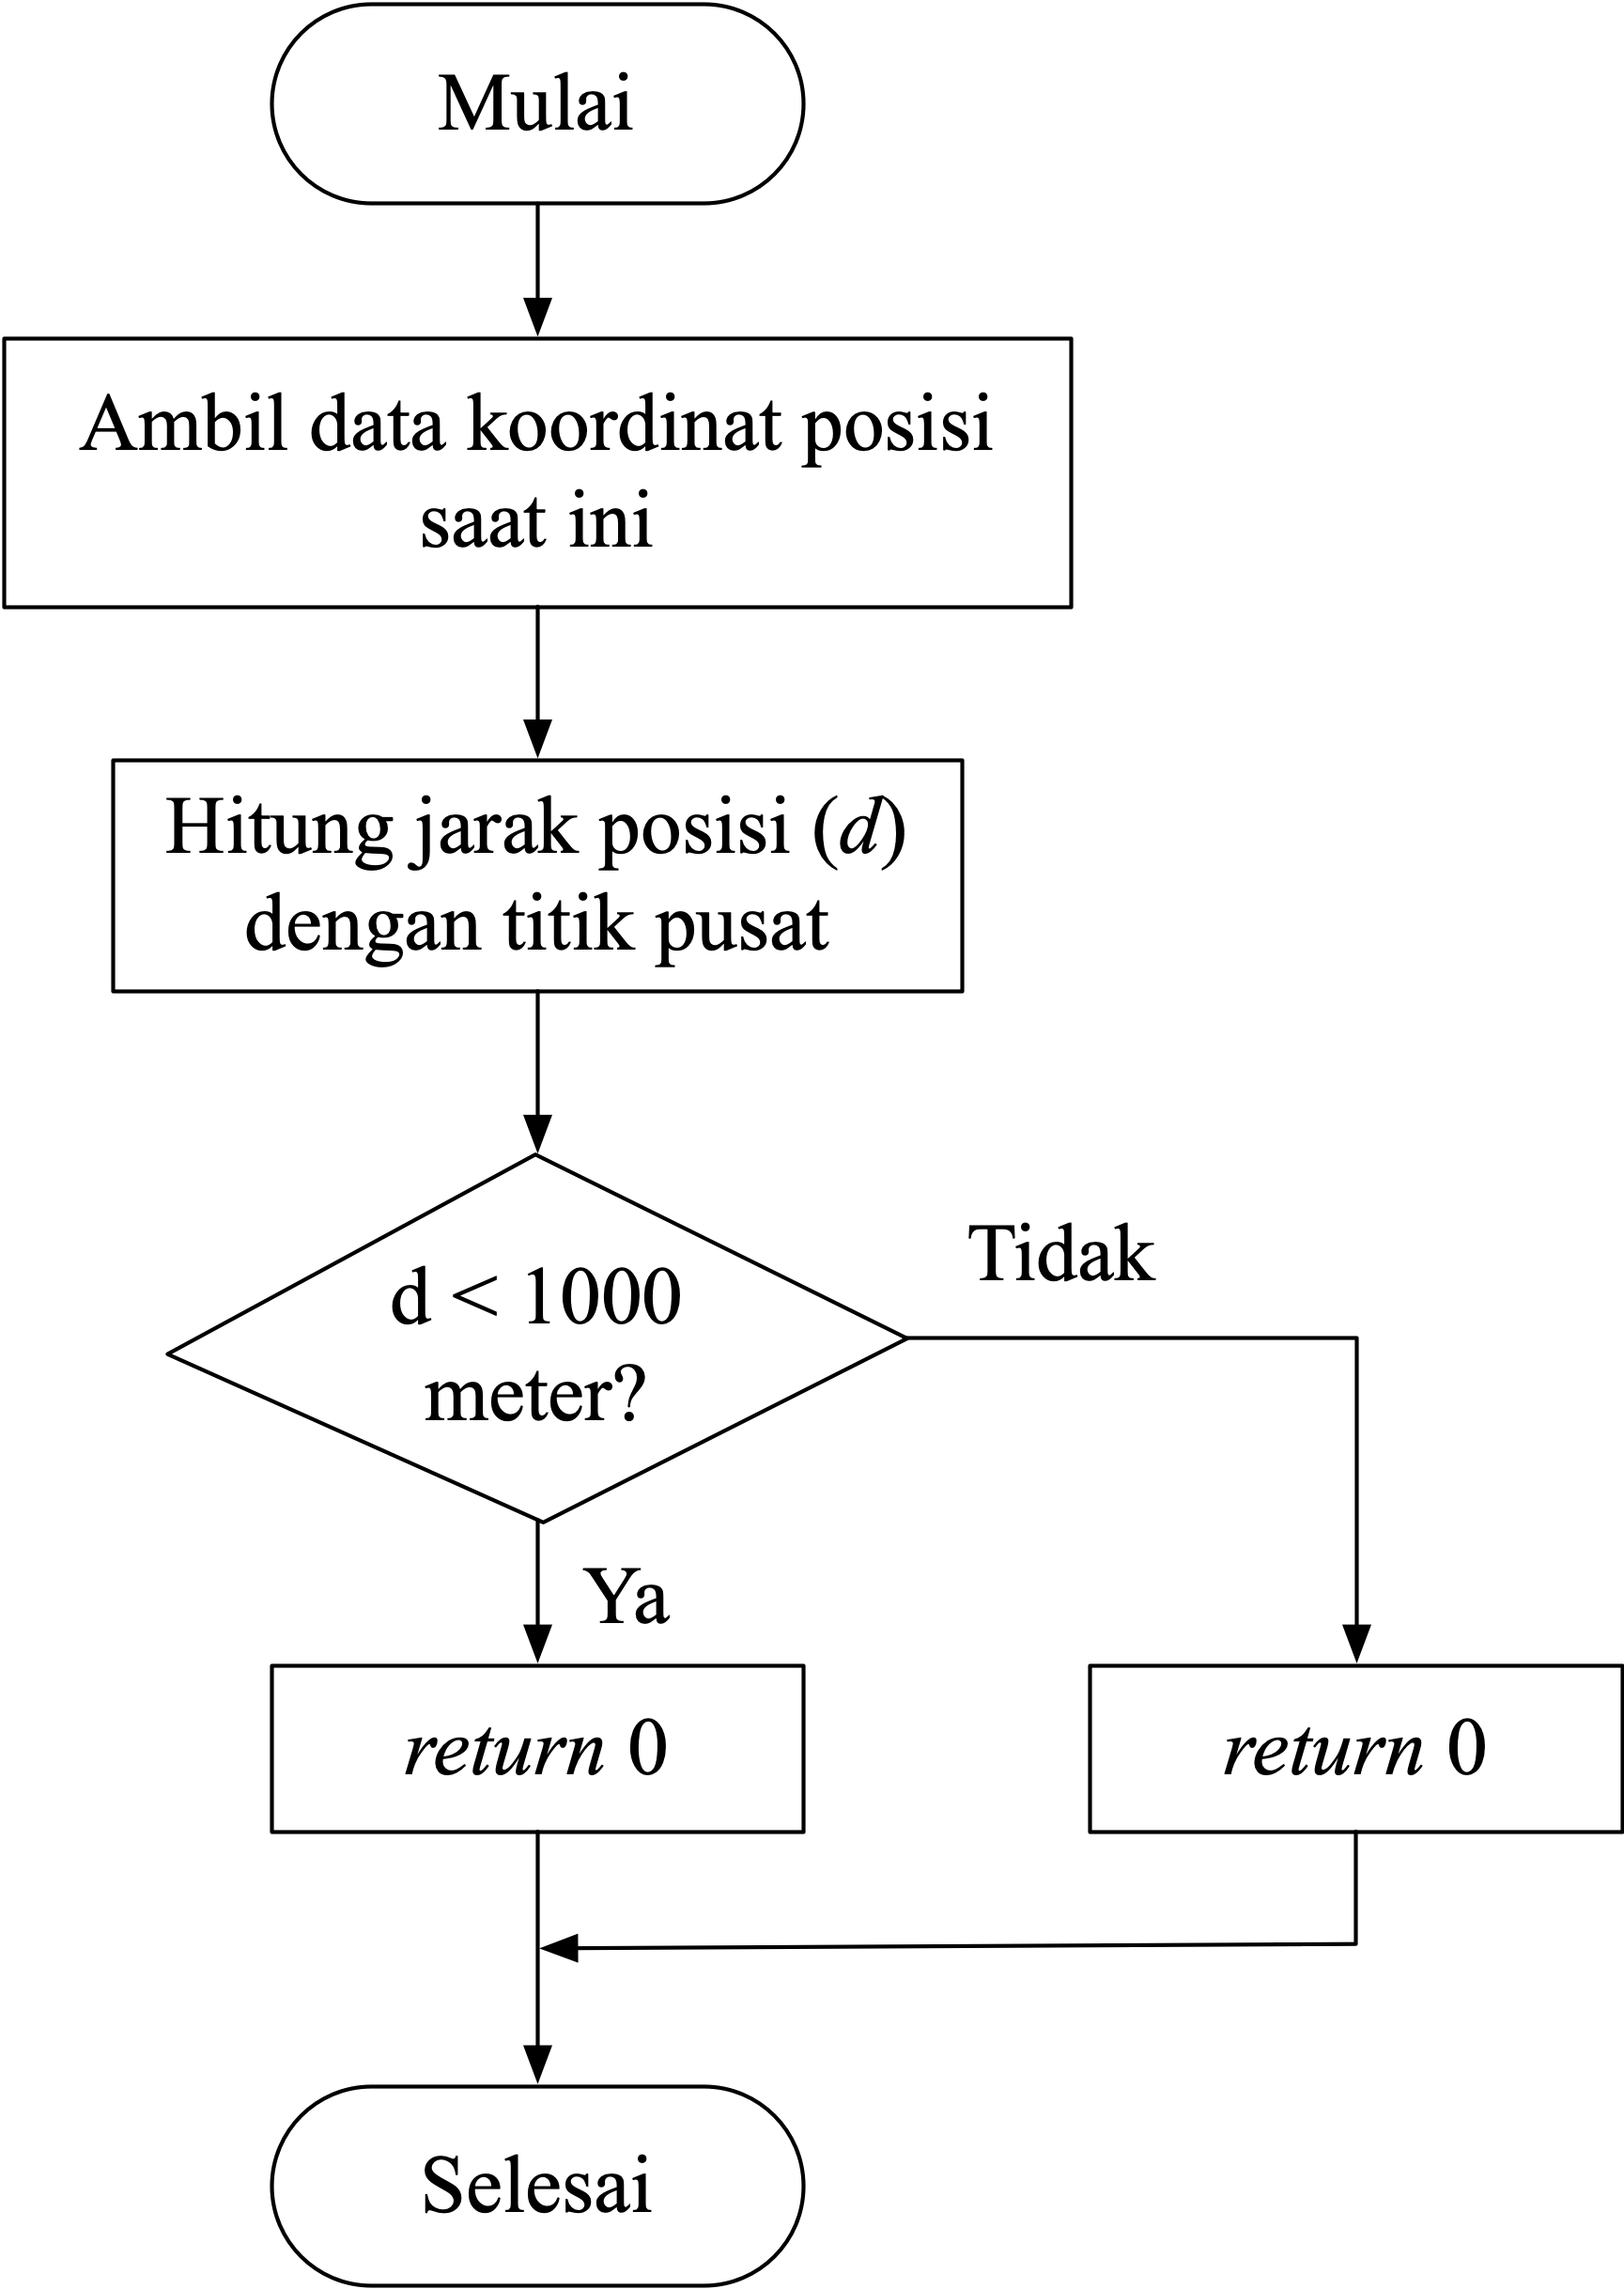
\includegraphics[width=8cm]{contents/chapter-3/flowchart-geofencing-ugm.png}
	\caption{Diagram Alir Fungsi \textit{Geofencing} Wilayah Universitas Gadjah Mada}
	\label{Fig: flowchart-geofencing-ugm}
\end{figure}

\section{Algoritma \textit{Geofencing}}
\subsection{\textit{Geofencing} Wilayah Universitas Gadjah Mada}
Perhitungan \textit{geofencing} dilakukan pada sisi mikrokontroler dengan menggunakan fungsi \texttt{Geofence\_Check()}. Fungsi ini membutuhkan dua buah argumen, yaitu \texttt{latitude} untuk koordinat garis lintang dan \texttt{longitude} untuk koordinat garis bujur. Kedua argumen dalam bentuk \textit{floating point}. Fungsi ini akan mengembalikan integer untuk menunjukan apakah koordinat yang diberikan berada di dalam lingkaran dari satu titik yang telah ditentukan. Gambar \ref{Fig: flowchart-geofencing-ugm} menunjukan diagram alir fungsi \textit{geofencing} di  wilayah Universitas Gadjah Mada. Pada penelitian ini, titik pusat lingkaran diatur pada koordinat (-7,771376; 110,377493) dengan jari-jari 1000 meter.

Tahap pertama yang dilakukan pada implementasi \textit{geofencing} adalah melakukan inisiasi struktur \texttt{ugm\_coordinate} yang berisi koordinat dari titik pusat lingkaran dan variabel \texttt{distance} yang akan digunakan untuk menyimpan hasil perhitungan jarak. Algoritma \ref{alg: 3-define-geof} menunjukan inisiasi koordinat titik pusat dilakukan dengan memasukkan nilai koordinat garis lintang dan garis bujur pada elemen \texttt{lat} dan \texttt{lon} struktur \texttt{ugm\_coordinate}.

\begin{algorithm}[H]
	\caption{Inisiasi Struktur \texttt{ugm\_coordinate}}
	\label{alg: 3-define-geof}
	\begin{algorithmic}[1]
	\State \textbf{Declare} ugm\_coordinate as Coords\_t
	\State \textbf{Declare} distance as float64\_t
	\\
	\State ugm\_coordinate.lat $\gets$ -7.771376
	\State ugm\_coordinate.lon $\gets$ 110.377493		
	\end{algorithmic}
\end{algorithm}

Konversi derajat ke radian diperlukan karena koordinat yang didapat dalam satuan derajat, sedangkan fungsi trigonometri seperti \texttt{sin}, \texttt{cos}, dan \texttt{tan} pada pustaka \texttt{math.h} menerima argumen dalam satuan radian. Fungsi  \texttt{degToRad} berfungsi untuk mengonversi sudut dari satuan derajat menjadi satuan radian. Konversi ini dilakukan dengan cara mengalikan nilai sudut dalam derajat dengan nilai $\pi$, kemudian hasilnya dibagi dengan 180$^{\circ}$. Berdasarkan Algoritma \ref{alg: 3-deg2rad}, fungsi \texttt{degToRad} diimplementasikan menggunakan \textit{preprocessor directive} \texttt{\#define}.

\begin{algorithm}[H]
	\caption{Konversi Derajat ke Radian}
	\label{alg: 3-deg2rad}
	\begin{algorithmic}[1]
	\State \textbf{Define} \textsc{degToRad}(\textit{angleInDegrees}) as \textit{(angleInDegrees)} $\times \pi / 180.0$
	\end{algorithmic}
\end{algorithm}

Selanjutnya, selisih dari koordinat garis bujur dan garis lintang disimpan pada variabel \texttt{dLon} dan \texttt{dLat} seperti ditunjukan oleh Algoritma \ref{alg: 3-selisih-koord}.

\begin{algorithm}[H]
	\caption{Selisih Koordinat Garis Lintang dan Garis Bujur}
	\label{alg: 3-selisih-koord}
	\begin{algorithmic}[1]
	\State \textbf{Declare} dLat as float64\_t
	\State \textbf{Declare} dLon as float64\_t
	\\
	\State dLat $\gets$ \textsc{degToRad}(ugm\_coordinate.lat) - \textsc{degToRad}(latitude)
	\State dLon $\gets$ \textsc{degToRad}(ugm\_coordinate.lon) - \textsc{degToRad}(longitude)		
	\end{algorithmic}
\end{algorithm}

Setelah kedua nilai selisih garis bujur dan garis lintang antara dua titik dihitung, maka dilakukan perhitungan jarak antara kedua titik menggunakan persamaan Haversine. Persamaan ini prinsip trigonometri dari segitiga bola untuk menghitung jarak antara dua titik pada permukaan bola. Persamaan Haversine menghasilkan jarak dalam satuan radian sehingga perlu dikonversi ke satuan jarak bumi dengan mengalikannya dengan jari-jari bumi. Potongan kode sumber di bawah menggunakan persamaan Haversine untuk menghitung nilai \texttt{a} yang merepresentasikan setengah kuadrat dari jarak antara dua titik pada permukaan bola. Nilai \texttt{a} kemudian digunakan untuk menghitung nilai \texttt{c} yang merepresentasikan jarak antara dua titik dalam satuan radian. Implementasi perhitungan jarak dengan persamaan Haversine ditunjukan oleh Algoritma \ref{alg: 3-compute-ac}.

\begin{algorithm}[H]
	\caption{Perhitungan Jarak Antara Dua Titik dengan Persamaan Haversine}
	\label{alg: 3-compute-ac}
	\begin{algorithmic}[1]
	\State \textbf{Declare} a as float64\_t
	\State \textbf{Declare} c as float64\_t
	\\
	\State a $\gets$ pow(sin(dLat / 2), 2) + pow(sin(dLon / 2), 2) * cos(latitude) * cos(longitude)
	\State c $\gets$ 2 * asin(sqrt(a))			
	\end{algorithmic}
\end{algorithm}

Terakhir, setelah jarak antara dua titik berhasil dihitung menggunakan persamaan Haversine dan disimpan pada variabel \texttt{distance}, maka nilai jarak tersebut akan dibandingkan dengan jarak \textit{geofence} yang telah ditetapkan sebelumnya. Jika jarak antara dua titik kurang dari jarak \textit{geofence}, yang pada penelitian ini adalah 1000 meter, maka fungsi akan mengembalikan nilai satu sebagai representasi bahwa titik berada di dalam lingkaran. Sebaliknya, jika jarak antara dua titik lebih besar atau sama dengan jarak \textit{geofence}, maka fungsi akan mengembalikan nilai nol seperti ditunjukan oleh Algoritma \ref{alg: 3-return-geof-ugm}.

\begin{algorithm}[H]
	\caption{\textit{Return Value} Fungsi \textit{Geofencing} Wilayah Universitas Gadjah Mada}
	\label{alg: 3-return-geof-ugm}
	\begin{algorithmic}[1]
	\If{distance $<$ 1000}
		\State \textbf{return} 1
	\Else
		\State \textbf{return} 0
	\EndIf	
	\end{algorithmic}
\end{algorithm}

\begin{figure}[H]
	\centering
	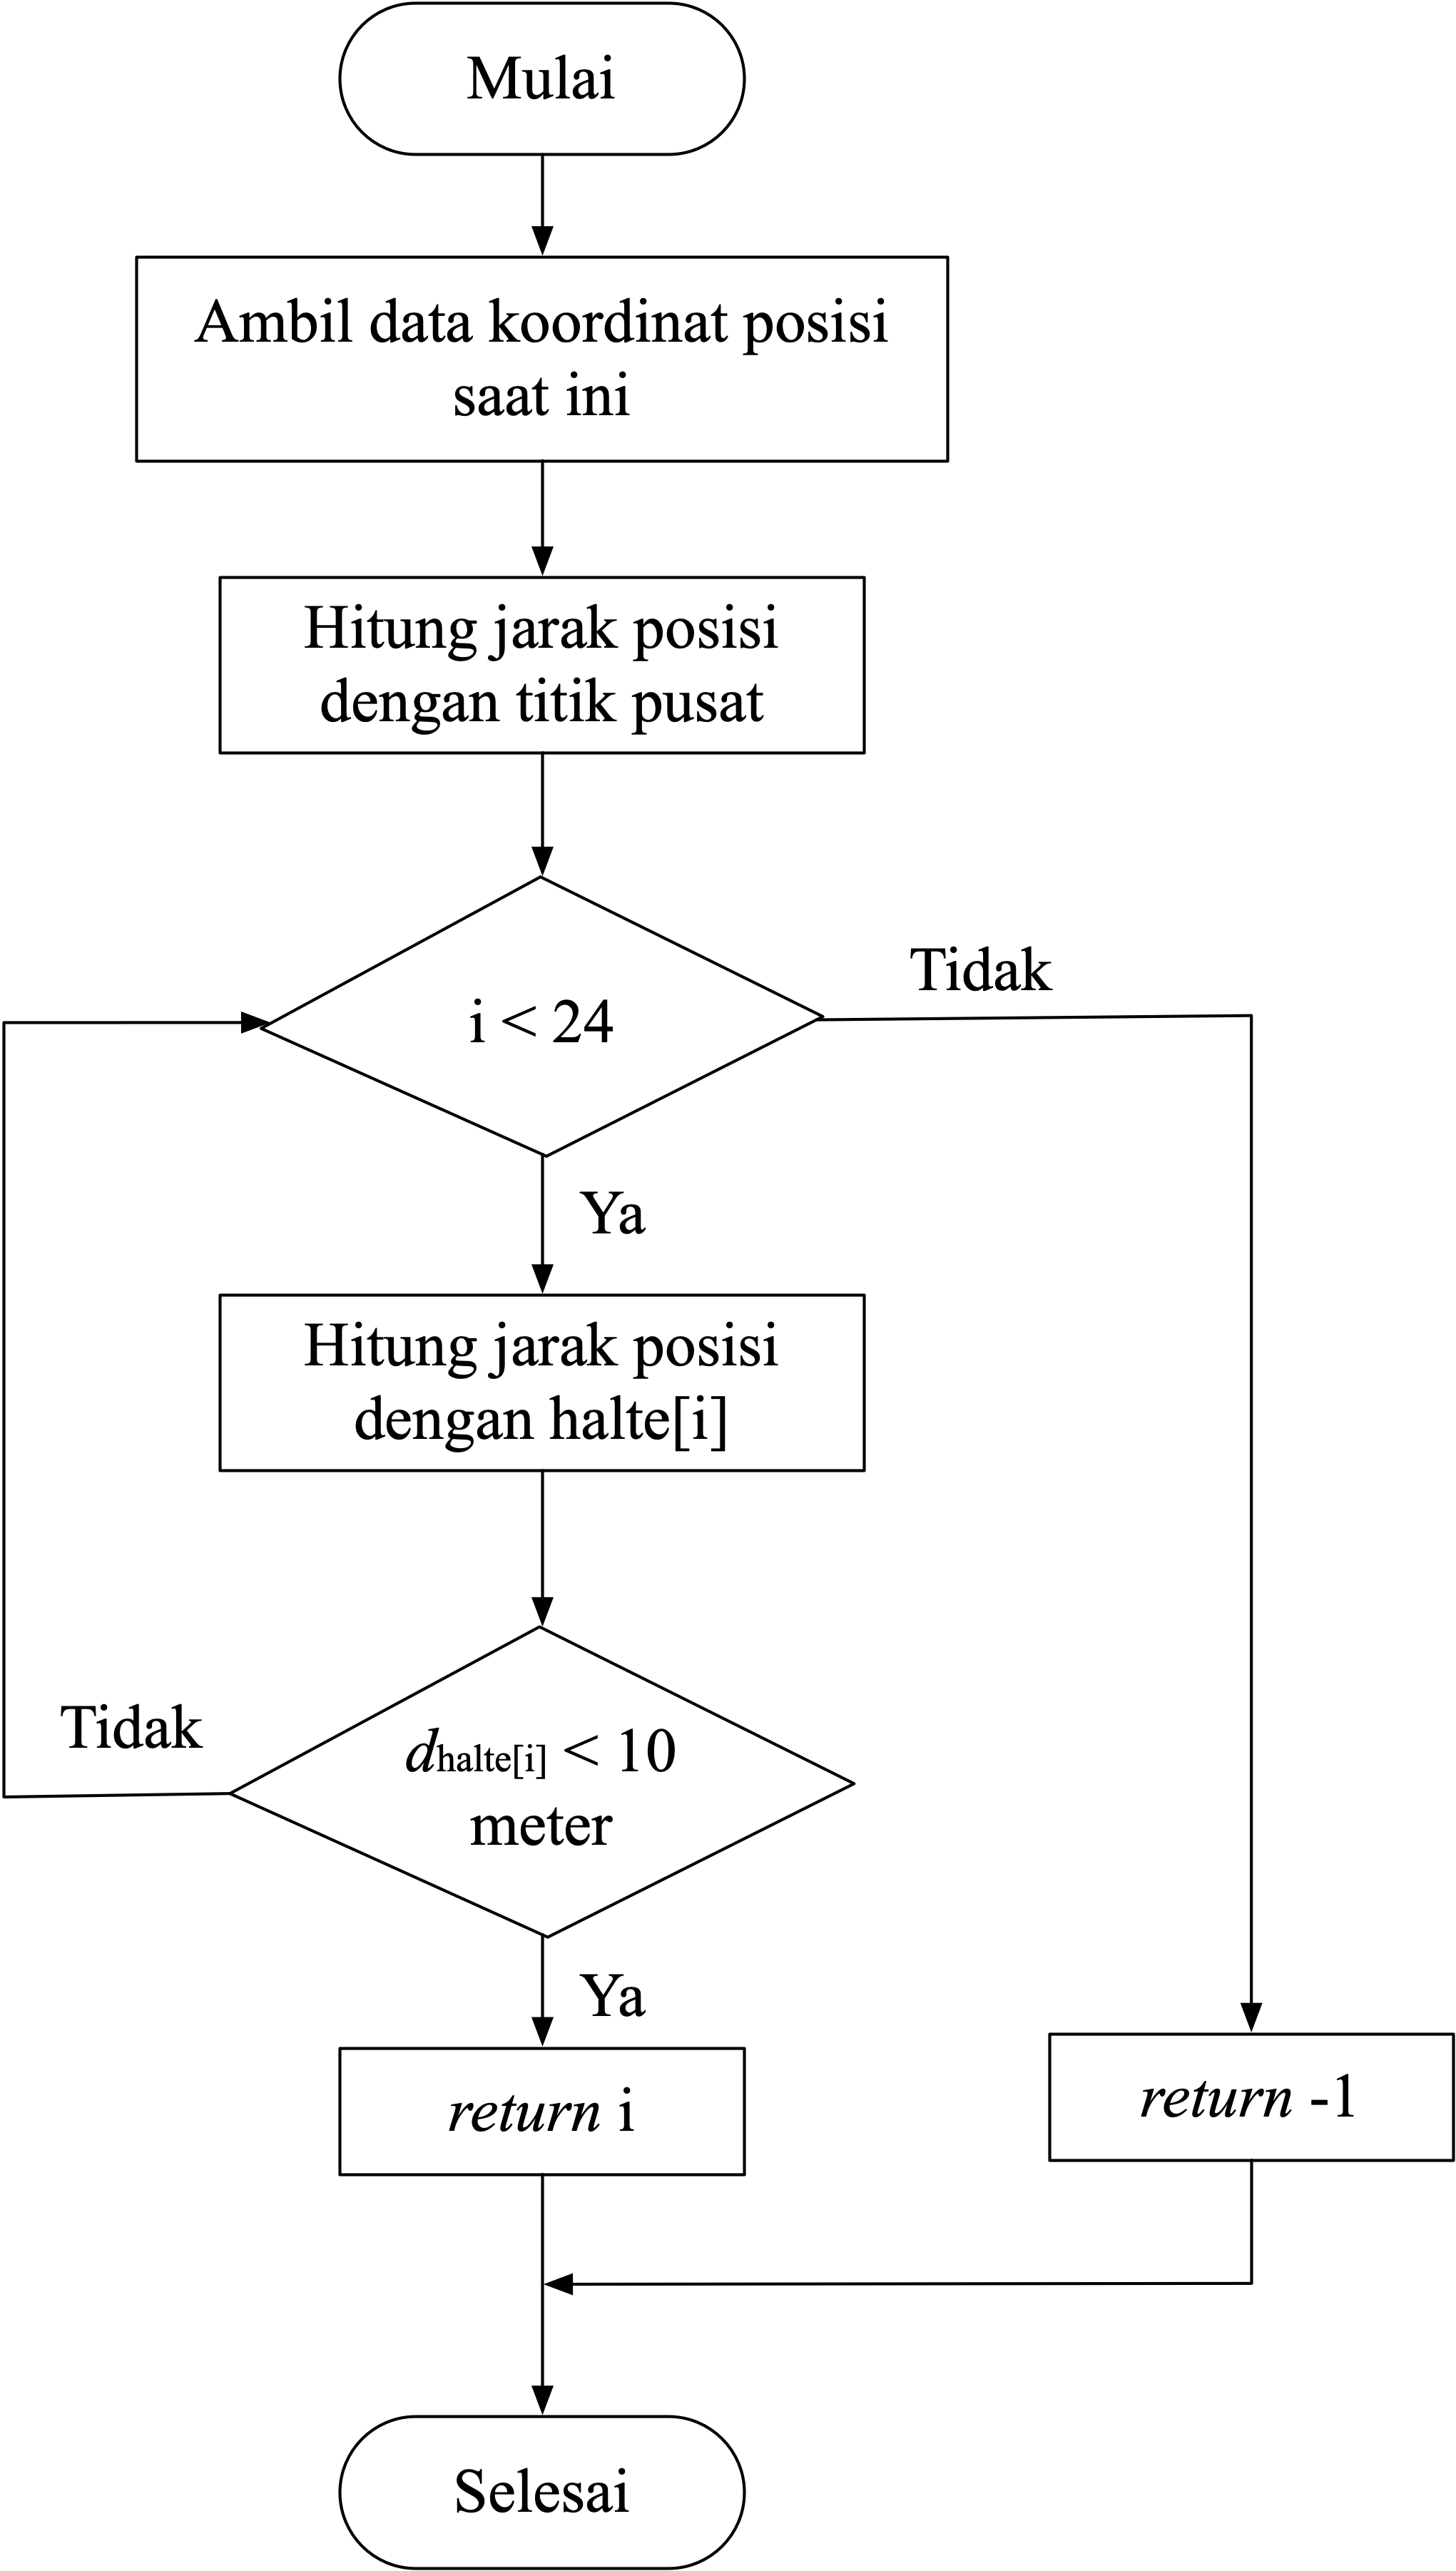
\includegraphics[width=9cm]{contents/chapter-3/flowchart-geofencing-halte.png}
	\caption{Diagram Alir Fungsi \textit{Geofencing} Halte}
	\label{Fig: flowchart-geofencing-halte}
\end{figure}

\subsection{\textit{Geofencing} Halte}
Selain untuk menentukan apakah bus berada di area Universitas Gadjah Mada atau tidak, algoritma \textit{geofencing} yang telah dirancang pada bagian sebelumnya dapat dikembangkan lebih lanjut untuk menentukan apakah bus sedang berhenti di satu halte atau tidak. Untuk menentukan apakah bus sedang berhenti di satu halte atau tidak maka digunakan fungsi \texttt{Stopped\_at\_Halte}. Gambar \ref{Fig: flowchart-geofencing-halte} menunjukan diagram alir proses pada \textit{geofencing} di halte Bus Trans Gadjah Mada. 

Fungsi tersebut menerima satu argumen dengan tipe data \texttt{Coords\_t}. Fungsi ini bekerja dengan cara menghitung jarak posisi saat ini terhadap setiap koordinat halte yang ada. Jika terdapat halte yang berjarak kurang dari lima meter, maka fungsi akan mengembalikan indeks halte dengan jarak kurang dari lima meter. Sebaliknya, jika tidak ditemukan halte dengan jarak kurang dari lima meter maka fungsi akan mengembalikan negatif satu. Implementasi dari fungsi ini ditunjukan oleh Algoritma \ref{alg: 3-geof-halte}.

\begin{algorithm}[H]
	\caption{Implementasi \textit{Geofencing} Halte}
	\label{alg: 3-geof-halte}
	\begin{algorithmic}[1]
	\Function{Stopped\_at\_Halte}{$location$}
		\State \textbf{Declare} $distance$ as float64\_t
		\State \textbf{Declare} $halte$ as Coords\_t
		\\
		\For{$i \gets 0$ to $HALTE\_COUNTS - 1$}
			\State $halte.lat \gets halte\_coords[0][i]$
			\State $_halte.lon \gets halte\_coords[1][i]$
			\\
			\State $distance \gets$ \Call{Calculate\_Distance}{$location, halte$}
			\\
			\If{$distance < 15$}
				\State \textbf{return} $i$
			\EndIf
		\EndFor
		\\
		\State \textbf{return} -1
	\EndFunction
	\end{algorithmic}
\end{algorithm}

Untuk meminimalisasi galat dan memastikan bahwa bus benar-benar berhenti di halte, maka \textit{firmware} akan memastikan bahwa posisi fiksasi bus terletak dalam radius halte tiga kali berturut-turut. Adapun implementasi dari bagian ini ditunjukan oleh Algoritma \ref{alg: 3-geof-halte-verif}.

\begin{algorithm}[H]
	\caption{Implementasi Verifikasi Halte Saat Ini}
	\label{alg: 3-geof-halte-verif}
	\begin{algorithmic}[1]
	\State \textbf{Declare} $prev\_stopped\_at\_halte$ as uint8\_t
	\State \textbf{Declare} $stop\_count$ as int
	\\
	\If{gpgga\_data.xyz.stopped\_at\_halte $<$ 0}
		\If{gpgga\_data.xyz.stopped\_at\_halte $=$ $prev\_stopped\_at\_halte$}
			\State $stop\_count \mathrel{+}= 1$
			\\
			\If{$stop\_count = 3$}
				\State \Call{sprintf}{(char *)msg, "\%d", gpgga\_data.xyz.stopped\_at\_halte}
				\State \Call{GNSS\_PRINT}{(char *)msg}
			\EndIf
		\Else
			\State $prev\_stopped\_at\_halte \gets$ gpgga\_data.xyz.stopped\_at\_halte
			\State $stop\_count \gets 0$
		\EndIf
	\EndIf		
	\end{algorithmic}
\end{algorithm}

\section{Menampilkan Hasil Penguraian}
Setelah proses penguraian dilakukan, tahap selanjutnya adalah menampilkan hasil penguraian pada \textit{serial monitor}. Pada \textit{firmware} ini, untuk menampilkan hasil penguraian dalam bentuk yang lebih mudah dibaca dapat dilakukan dengan mengatur nilai \texttt{GNSS\_READABLE} dengan nilai satu. Contoh keluaran jika nilai \texttt{GNSS\_READABLE} diatur menjadi satu ditunjukan oleh \textit{listing} di bawah.

\vspace{0.3cm}
\begin{lstlisting}[style=mystyle]
	UTC   : 02:01:01
	LAT   : -7.768369
	LON   : 110.385078
	ALT   : 205.0
	SATS  : 11
	HDOP  : 0.9
	VDOP  : 1.8
	PDOP  : 2.0
	HALTE : 4
	GEOF  : 1
\end{lstlisting}

Format di atas dirancang sedemikian rupa untuk memudahkan membaca hasil penguraian oleh manusia. Di sisi lain, untuk memudahkan pengolahan data hasil pengujian, hasil penguraian ditampilkan dalam format \textit{comma seperated values} atau CSV. Untuk menampilan dalam mode CSV, nilai \texttt{GNSS\_READABLE} diatur menjadi nol. Contoh dari keluaran dalam format CSV ditunjukan oleh \textit{listing} di bawah.

\vspace{0.3cm}
\begin{lstlisting}[style=mystyle]
02:10:30,-7.771091,110.38131,5.0,185.9,2.3,14,1.0
\end{lstlisting}

Setiap nilai dipisahkan oleh koma (,) dan tidak ada spasi yang digunakan. Urutan nilai yang ditampilkan adalah: waktu UTC, koordiat garis lintang, koordinat garis bujur, visibilitas satelit, ketinggian, akurasi posisi (HDOP), keluaran \textit{geofencing} halte, dan keluaran \textit{geofencing} wilayah Universitas Gadjah Mada. Format CSV digunakan karena dapat memudahkan pengolahan data hasil pengujian karena format ini memungkinkan data untuk disimpan dalam bentuk teks sederhana yang dapat dengan mudah dibaca dan diproses oleh program komputer seperti Excel atau Python.

Untuk menampilkan ke \textit{serial monitor}, digunakan fungsi \texttt{GNSS\_PRINT} untuk menyederhanakan proses penampilan. Adapun implementasi dari fungsi \texttt{GNSS\_PRINT} ditunjukan oleh Algoritma \ref{alg: 3-gnss-print}.

\begin{algorithm}[H]
	\caption{Function \texttt{GNSS\_PRINT}}
	\label{alg: 3-gnss-print}
	\begin{algorithmic}[1]
		\Function{GNSS\_PRINT}{$pBuffer$}
			\If{\Call{HAL\_UART\_Transmit} $\neq$ HAL\_OK}
				\State \textbf{return} 1
			\EndIf
			\State \Call{fflush}{stdout}
			\State \textbf{return} 0
		\EndFunction
	\end{algorithmic}
\end{algorithm}

Tujuan dari fungsi di atas adalah untuk menampilkan data pada \textit{serial monitor} dengan mengirimkan data ke UART. Fungsi ini memiliki satu parameter input yaitu \texttt{pBuffer} yang berupa \textit{pointer} ke \texttt{char} yang menyimpan data yang akan ditampilkan pada \textit{serial monitor}.

Pertama, fungsi \texttt{HAL\_UART\_Transmit} dipanggil dengan parameter yang terdiri dari alamat \texttt{hcom\_uart[COM1]} yang merupakan sebuah \textit{handle} UART, \textit{pointer} ke \texttt{pBuffer} yang berisi data yang akan dikirimkan, panjang data yang akan dikirimkan yaitu \texttt{strlen((char *)pBuffer)}, dan \textit{timeout} sebesar 1000 milisekon. Fungsi ini akan mencoba untuk mengirimkan data ke UART dan mengembalikan nilai \texttt{HAL\_OK} jika pengiriman berhasil dilakukan. Sebaliknya, jika pengiriman data tidak berhasil, fungsi akan mengembalikan nilai 1.

Setelah itu, \texttt{fflush(stdout)} dipanggil untuk membersihkan \textit{output buffer} pada \textit{stdout}, yaitu standar keluaran yang biasanya digunakan untuk menampilkan data pada layar komputer. Hal ini dilakukan untuk memastikan bahwa data sudah tercetak pada \textit{serial monitor}.

Fungsi kemudian mengembalikan nilai 0 jika pengiriman data berhasil dilakukan dan mengembalikan nilai 1 jika pengiriman tidak berhasil dilakukan. Nilai kembalian fungsi ini dapat digunakan sebagai penanda keberhasilan atau kegagalan pengiriman data.

\section{Pengolahan Data}
Pengolahan data dari hasil pengujian sistem adalah salah satu bagian penting untuk meninjau performa dari sistem. Dalam pengolahan data GNSS, salah satu alat yang sering digunakan adalah bahasa pemrograman Python. Bahasa pemrograman Python dipilih karena merupakan salah satu bahasa paling populer di bidang analisis data dan memiliki komunitas yang sangat besar. Hal tersebut membuat banyak pengembang merancang berbagai pustaka untuk pengolahan data termasuk data dari modul GNSS. Dengan menggunakan bahasa pemrograman Python diharapkan dapat mempermudah dan mempercepat proses pengolahan data. Pada bagian ini akan dibahas cara mengolah data baik dari modul GNSS secara langsung maupun yang telah diolah oleh \textit{firmware} yang telah dirancang pada bagian sebelumnya.

\subsection{Modul GNSS}
Hasil pengujian pada modul GNSS berupaka sekumpulan kalimat NMEA yang disimpan dalam satu \textit{file} teks. Tentunya kalimat NMEA yang didapat memuat berbagai informasi penting mengenai performa modul Teseo\hyp{}LIV3FL. Pada pengolahan data pengujian ini akan digunakan enam pustaka, yaitu Pandas, NumPy, PyNMEA2, Matplotlib, dan Seaborn. Pandas digunakan untuk mengolah dan analisis data, sementara NumPy menyediakan struktur data untuk operasi numerik pada data. PyNMEA2 digunakan untuk penguraian kalimat NMEA yang dihasilkan oleh modul GNSS. Matplotlib dan Seaborn digunakan untuk pembuatan visualisasi data. Matplotlib menyediakan berbagai fungsi untuk membuat plot, termasuk plot waktu dan plot \textit{scatter}. Sementara Seaborn memungkinkan pembuatan plot dengan tampilan yang lebih menarik dan interaktif. Selain itu, terdapat perintah untuk mengimpor modul dari Matplotlib seperti \texttt{FuncFormatter} dan \texttt{MaxNLocator} yang digunakan untuk mengatur tampilan sumbu pada plot.

Setelah memuat seluruh pustaka yang digunakan, langkah selanjutnya adalah melakukan konfigurasi parameter untuk visualisasi data Matplotlib. Pertama, objek \textit{formatter} dibuat dengan format tanggal dan waktu pada variabel \texttt{myFmt}. Adapun format yang digunakan adalah \texttt{\%H:\%M:\%S}, yang menunjukkan jam, menit, dan detik. Selanjutnya, untuk meningkatkan resolusi gambar maka resolusi DPI pada gambar dapat diatur dengan \texttt{mpl.rcParams['figure.dpi'] = 300.} Semakin tinggi nilai DPI, semakin berkualitas tampilan gambar yang dihasilkan. Terakhir, pengaturan \textit{font} dilakukan agar grafik yang didapat menggunakan \textit{font} Times New Roman. Bagian konfigurasi Matplotlib ditunjukan oleh Algoritma \ref{alg: 3-mpl-config}.

\begin{algorithm}[H]
	\caption{Konfigurasi Tampilan Matplotlib}
	\label{alg: 3-mpl-config}
	\begin{algorithmic}[1]
	\State $myFmt \gets$ \textsc{mdates.DateFormatter}(``\%H:\%M:\%S'') 
	\\
	\State mpl.rcParams['figure.dpi'] $\gets$ 300
	\State plt.rcParams["font.family"] $\gets$ ``Times New Roman''
	\State plt.rcParams["mathtext.fontset"] $\gets$ ``dejavuserif''		
	\end{algorithmic}
\end{algorithm}

Terakhir, digunakan fungsi \texttt{pd.read\_csv()} untuk membaca \textit{file} teks kalimat NMEA hasil pengamatan. Argumen \texttt{head} diatur sebagai \texttt{None} untuk menandakan bahwa pada \textit{file} teks tidak terdapat \textit{header}. Kemudian, argumen \texttt{sep} diisi dengan " 
" untuk menunjukan setiap kolom dipisahkan dengan spasi. Terakhir, argumen \texttt{encoding} diatur sebagai \texttt{unicode\_escape} untuk menangani karakter spesial seperti \textit{backslash}.

\subsubsection{Ketelitian dari Teseo\hyp{}LIV3FL}
Langkah awal yang dilakukan untuk meninjau ketelitian dari modul GNSS Teseo\hyp{}LIV3FL adalah dengan inisiasi \textit{DataFrame} \texttt{teseo\_accuracy\_df} yang memiliki empat kolom, yaitu (\texttt{timestamp}, \texttt{pdop}, \texttt{hdop}, dan \texttt{vdop}). Selanjutnya, program akan melakukan iterasi pada setiap kalimat NMEA. Pada bagian ini, kalimat NMEA yang akan digunakan adalah GPGGA dan GNGSA. Implementasi dari pengolahan data ketelitian dari modul Teseo\hyp{}LIV3FL ditunjukan oleh Algoritma \ref{alg: 3-gpgga-pyparse}.

\begin{algorithm}[H]
	\caption{\textit{Parsing} Kalimat \$GPGGA pada Python}
	\label{alg: 3-gpgga-pyparse}
	\begin{algorithmic}[1]
	\For{$i$ in range(0, GNGSA.size)}
		\State $parser \gets$ \textsc{pynmea2.parse}(GNGSA['msg'].iloc[i])
		\\
		\If{GNGSA.msg.iloc[i].startswith("\$GPGGA")}
		\State $timestamp \gets$ parser.timestamp
		\Else
		\State $hdop \gets$ \textsc{float}(parser.hdop)
		\State $vdop \gets$ \textsc{float}(parser.vdop)
		\State $pdop \gets$ \textsc{float}(parser.pdop)
		\\
		\State $temp \gets$ \textsc{pd.DataFrame}({'timestamp':timestamp, 'pdop':pdop, 'hdop':hdop, 'vdop':vdop}, index=[i])
		\\
		\State $teseo\_accuracy\_df \gets$ \textsc{pd.concat}([teseo\_accuracy\_df, temp], axis=0)
		\EndIf
	\EndFor		
	\end{algorithmic}
\end{algorithm}

Jika kalimat NMEA dimulai dengan "\$GPGGA" maka program akan menyimpan nilai waktu dari kalimat tersebut ke dalam variabel \texttt{timestamp}. Di sisi lain, jika kalimat NMEA tidak diawali dengan "\$GPGGA", maka program akan menyimpan nilai hdop, vdop, dan pdop dari kalimat tersebut ke dalam variabel \texttt{hdop}, \texttt{vdop}, dan \texttt{pdop} secara berturut-turut. Selanjutnya, program akan membuat \textit{DataFrame} sementara yang berisi nilai waktu UTC, PDOP, HDOP, dan VDOP yang didapatkan dari kalimat NMEA tersebut. \textit{DataFrame} sementara tersebut akan digabungkan dengan \textit{DataFrame} utama, yaitu \texttt{teseo\_accuracy\_df} menggunakan metode \texttt{pd.concat()}.

Untuk mendapatkan nilai CEP maka diperlukan nilai standar deviasi pada kedua koordinat garis bujur dan garis lintang. Dua informasi tersebut dapat diperoleh pada kalimat NMEA \$GPGST. Kemudian, dilakukan iterasi sebanyak jumlah baris data di dalam objek DataFrame \texttt{sats\_gst\_raw\_df}. Pada setiap iterasi, dilakukan penguraian data NMEA dengan menggunakan fungsi \texttt{pynmea2.parse()} dan disimpan ke dalam variabel \texttt{parser}. Data-data yang diperlukan diambil dari objek parser, yaitu \texttt{std\_dev\_x} dan \texttt{std\_dev\_y }serta dihitung nilai CEP-nya. Selanjutnya, data hasil penguraian tersebut disimpan ke dalam sebuah objek \textit{DataFrame} sementara bernama \texttt{temp} dengan index yang sesuai dengan nomor iterasi. Objek \texttt{temp} tersebut kemudian digabungkan dengan objek DataFrame \texttt{sats\_gst\_df} menggunakan metode \texttt{pd.concat()} untuk menyusun \textit{DataFrame} baru. Implementasi dari perhitungan CEP ditunjukan oleh Algoritma \ref{alg: 3-gst-pyparse}.

\begin{algorithm}[H]
	\caption{\textit{Parsing} Kalimat \$GNGSA pada Python}
	\label{alg: 3-gst-pyparse}
	\begin{algorithmic}[1]
	\For{$i$ in range(0, sats\_gst\_raw\_df.size)}
		\State $parser \gets$ \textsc{pynmea2.parse}
		\\
		\State $timestamp \gets$ parser.timestamp
		\State $rms \gets$ parser.rms
		\State $std\_dev\_x \gets$ parser.std\_dev\_longitude
		\State $std\_dev\_y \gets$ parser.std\_dev\_latitude
		\State $std\_dev\_z \gets$ parser.std\_dev\_altitude
		\State $drms \gets \sqrt{std\_dev\_x^2 + std\_dev\_y^2}$
		\\
		\State $cep \gets (0.62 \times std\_dev\_x) + (0.56 \times std\_dev\_y)$
		\\
		\State $temp \gets$ \textsc{pd.DataFrame}({"timestamp": timestamp, "rms": rms, "std\_dev\_x": std\_dev\_x, "std\_dev\_y": std\_dev\_y, "std\_dev\_z": std\_dev\_z, "drms": drms, "cep": cep}, index=[i])
		\\
		\State $sats\_gst\_df \gets$ \textsc{pd.concat}([sats\_gst\_df, temp], axis=0)
	\EndFor
	\end{algorithmic}
\end{algorithm}

\subsubsection{Visibilitas Satelit}
Untuk meninjau visibilitas satelit maka digunakan kalimat NMEA \$GPGGA dan \$GNGSA. Program akan melakukan iterasi sebanyak jumlah kalimat \$GPGGA dan \$GNGSA. Jika kalimat tersebut dimulai dengan "\$GPGGA", maka waktu akan diambil dari objek \texttt{parser}. Jika tidak, maka program akan mengambil informasi mengenai PRN, \textit{azimuth}, \textit{elevation}, dan SNR dari setiap satelit. Selanjutnya, program membuat \textit{DataFrame} baru dengan kolom \texttt{timestamp}, \texttt{prn}, \texttt{azimuth}, \texttt{elevation}, dan \texttt{snr} yang diambil dari objek parser untuk empat satelit. \textit{DataFrame} baru ini akan ditambahkan ke \textit{DataFrame} \texttt{sats\_detail\_info\_df} menggunakan fungsi \texttt{concat()}. Implementasi dari penguraian data satelit ditunjukan oleh Algoritma \ref{alg: 3-sats-parse}.

\begin{algorithm}[H]
	\caption{\textit{Parsing} Informasi Satelit pada Python}
	\label{alg: 3-sats-parse}
	\begin{algorithmic}[1]
	\State $timestamp \gets \text{None}$
	\State $time \gets \text{None}$
	\State $sats\_detail\_info\_df \gets \text{empty DataFrame}$
	\\
	\For{$i$ \textbf{in range} $(sats\_string\_df.size)$}
		\State $parser \gets \text{pynmea2.parse}(sats\_string\_df.msg.iloc[i])$
		\If{$sats\_string\_df.msg.iloc[i]$ \textbf{startswith} "$GPGGA$"}
		\State $time \gets parser.timestamp$
		\Else
		\If{$timestamp$ \textbf{is None}}
		\State $timestamp \gets [time] \times 4$
		\EndIf
		\State $PRN \gets PRN_n$
		\State $Azimuth \gets Azimuth_n$
		\State $Elevation \gets Elevation_n$
		\State $SNR \gets SNR_n$
		\State $temp \gets \text{DataFrame}({timestamp, PRN, Azimuth, Eleation, SNR})$
		\State $sats\_detail\_info\_df \gets \text{concatenate}(sats\_detail\_info\_df, temp)$
		\EndIf
	\EndFor
	\end{algorithmic}
\end{algorithm}
	
Dalam standar NMEA 3.10, setiap konstelasi memiliki rentang PRN yang berbeda-beda dan tidak tumpang tindih. Satelit pada konstelasi GPS memiliki PRN dari 1 hingga 32, SBAS memiliki PRN dari 33 hingga 51, GLONASS memiliki PRN dari 65 hingga 92, BeiDou memiliki PRN dari 141 hingga 172, QZSS memiliki PRN dari 183 hingga 197, sementara Galileo memiliki PRN dari 301 hingga 330. Untuk visualisasi jumlah satelit dan pergerakannya di \textit{sky plot} maka perlu dipisahkan setiap konstelasi berdasarkan nilai PRN-nya.

Proses ini diawali dengan inisialisasi variabel \texttt{gps}, \texttt{beidou}, \texttt{qzss}, \texttt{galileo}, dan \texttt{total} dengan nilai awal sebesar nol. Selanjutnya, dilakukan pengelompokan data pada \texttt{sats\_detail\_info\_df} untuk memperoleh data satelit yang terdeteksi pada waktu tertentu dan disimpan dalam variabel \texttt{sats}. Kemudian dilakukan penghitungan jumlah satelit untuk masing-masing sistem navigasi satelit (GPS, Beidou, QZSS, Galileo) berdasarkan nomor PRN dari satelit yang terdeteksi pada waktu tersebut. Jika nomor PRN satelit berada pada rentang nilai tertentu, maka dihitung sebagai jumlah satelit pada sistem navigasi satelit tersebut. Terakhir, jumlah seluruh satelit dihitung dengan menjumlahkan jumlah satelit pada setiap konstelasi setiap waktunya. Implementasi dari pengelompokan satelit ditunjukan oleh potongan Algoritma \ref{alg: 3-sats-count}.

\begin{algorithm}[H]
	\caption{Menghitung Jumlah Satelit untuk Setiap Konstelasi pada Python}
	\label{alg: 3-sats-count}
	\begin{algorithmic}[1]
	\For{$timestamp$ \textbf{in} $timestamps$}
	\State $gps, beidou, qzss, galileo, total \gets 0, 0, 0, 0, 0$
	\\
	\For{$i$ \textbf{in range} $(0, sats.\text{timestamp}.\text{count}())$}
	\If{$sats.\text{iloc}[i].prn < 52$ \textbf{and} $sats.\text{iloc}[i].prn > 0$}
	\State $gps \gets gps + 1$
	\EndIf
	\If{$sats.\text{iloc}[i].prn < 173$ \textbf{and} $sats.\text{iloc}[i].prn > 140$}
	\State $beidou \gets beidou + 1$
	\EndIf
	\If{$sats.\text{iloc}[i].prn < 199$ \textbf{and} $sats.\text{iloc}[i].prn > 181$}
	\State $qzss \gets qzss + 1$
	\EndIf
	\If{$sats.\text{iloc}[i].prn < 332$ \textbf{and} $sats.\text{iloc}[i].prn > 299$}
	\State $galileo \gets galileo + 1$
	\EndIf
	\State $total \gets gps + beidou + qzss + galileo$
	\EndFor
	\EndFor
	\end{algorithmic}
\end{algorithm}

\iffalse
\subsubsection{Eksplorasi SNR}
Selain visibilitas satelit dan DOP, SNR atau \textit{Signal-to-Noise} merupakan salah satu indikator kualitas data konstelasi GNSS. Nilai SNR menunjukan rasio antara daya isyarat pembawa dengan derau. Daya isyarat pembawa merupakan isyarat yang dikirimkan oleh satelit GNSS dan diterima oleh modul GNSS, sedangkan derau merupakan gangguan atau interferensi yang terjadi dalam proses transmisi isyarat tersebut. Dapat dikatakan bahwa semakin besar nilai SNR maka semakin baik kualitas isyarat yang diterima oleh modul GNSS. Nilai SNR direpresentasikan dengan satuan desibel-Hertz atau dBHz.

Untuk mendapatkan nilai PRN dari setiap konstelasi, setiap satelit akan dikelompokan berdasarkan stander NMEA 3.10 yang telah dijelaskan pada bagian sebelumnya. Proses pengelompokkan dilakukan dengan mengambil rentang nomor PRN untuk setiap konstelasi, kemudian memeriksa setiap satelit dalam \textit{DataFrame} \texttt{ sats\_detail\_info\_df} yang termasuk dalam rentang tersebut. Data satelit yang sudah dikelompokkan kemudian dihitung rata-rata, median, dan standar deviasi dari nilai SNR-nya. Hasil pengelompokkan setiap satelit berdasarkan konstelasi dan informasi rinci mengenai kualitas isyaratnya disimpan dalam variabel \texttt{grouped\_by\_prn}. Implementasi dari pengelompokan dan komputasi statistik dari nilai SNR untuk setiap konstelasi ditunjukan oleh Algoritma \ref{alg: 3-sats-prn}.

\vspace{0.3cm}
\begin{lstlisting}[language=python, style=mystyle, caption={Mengelompokan Satelit Berdasarkan PRN-nya pada Python}, label={lst: 3-sats-prn}]
grouped_by_prn = {}

for constellation in constellations:
	prn_range = constellation["prn_range"]
	
	sats_by_range = sats_detail_info_df[
		(sats_detail_info_df['prn'] > prn_range[0]) & 
		(sats_detail_info_df['prn'] < prn_range[1])
	]
	
	grouped_by_prn[constellation["title"]] = sats_by_range.groupby('prn')['snr'].agg(['mean', 'median', 'std'])
\end{lstlisting}
\fi

\subsection{Pengujian Sistem}
Pada subbab Pengembangan \textit{Firmware} bagian menampilkan hasil penguraian telah dijelaskan bahwa disediakan dua mode yang dapat diatur melalui nilai dari variabel \texttt{GNSS\_READABLE}. Format \texttt{GNSS\_READABLE} dikhususkan untuk mempermudah pemahaman seluruh keluaran hasil perhitungan pada sistem.

Untuk mempermudah proses mengolah data maka digunakan format data CSV. Pemilihan format data CSV dikarenakan formatnya yang sederhana sehingga dapat mempermudah proses eksplorasi data hasil pengujian sistem secara keseluruhan. Untuk mengatur \textit{firmware} agar keluaran data dalam bentuk CSV maka variabel \texttt{GNSS\_READABLE} diatur menjadi nol.

Selain itu, digunakan juga pustaka Folium untuk melukiskan koordinat pada peta. Pustaka Folium memungkinkan untuk \textit{plot} dengan variasi warna terhadap nilai dari satu parameter yang ingin ditinjau. Algoritma \ref{alg: 3-plot-hdop} di bawah adalah kode untuk \textit{plot} koordinat pengujian Bus Trans Gadjah Mada Rute 1B dengan variasi warna bergantung terhadap nilai HDOP pada titik tersebut.

\begin{algorithm}[H]
	\caption{\textit{Plot} Nilai HDOP di Setiap Titik Menggunakan Pustaka Folium}
	\label{alg: 3-plot-hdop}
	\begin{algorithmic}[1]
		\State lit\_coordinate = [-7.769711, 110.377441]
		\State mymap = folium.Map(location=lit\_coordinate, zoom\_start=15)
		\\
		\For{$i$ in range(0, len(df))}
			\State coords = [df.latitude[i], df.longitude[i]]
			\State hdop = df.hdop[i]
			\\
			\If{0 <= hdop < 1}
				\State color = dop\_cmap[0]
			\ElsIf{1 <= hdop < 2}
				\State color = dop\_cmap[1]
			\ElsIf{2 <= hdop < 5}
				\State color = dop\_cmap[2]
			\ElsIf{5 <= hdop < 10}
				\State color = dop\_cmap[3]
			\ElsIf{10 <= hdop < 20}
				\State color = dop\_cmap[4]
			\Else
				\State color = dop\_cmap[5]
			\EndIf
		\EndFor
		\\
		\State mymap.fit\_bounds([sw, ne]) 
		\\
		\State mymap		
	\end{algorithmic}
\end{algorithm}